\documentclass[11pt,b5paper,headings=small]{scrartcl}
\usepackage{graphicx}
\setkeys{Gin}{width=\columnwidth}
\usepackage[utf8]{inputenc}
\usepackage[T1]{fontenc}
\usepackage{libertine}
\usepackage[spacing,tracking]{microtype}
\microtypecontext{spacing=nonfrench}

\usepackage{caption}
\captionsetup{labelfont       = {bf, sf}}
\usepackage{float}
%%%
%%%

\let\origtextfloatsep\textfloatsep
\setlength{\textfloatsep}{5.5pt}
\setlength{\intextsep}{5.5pt}
\setlength{\abovecaptionskip}{5.5pt}

% Levels 
% I. 		section
% A.		subsection
% 1. 		subsubsection

\renewcommand*{\thesection}{\Roman{section}}
\renewcommand*{\thesubsection}{\Alph{subsection}}
\renewcommand*{\thesubsubsection}{\arabic{subsubsection}}

\renewcommand{\labelenumi}{\alph{enumi}.}

\addtokomafont{section}{\centering\large}
\addtokomafont{subsubsection}{\mdseries\scshape}

\begin{document}
\begin{center}
\LARGE US v Google%\\[0.75\baselineskip]

%\Large US Department of Justice
\end{center}
\iffalse
%%%
IN THE UNITED STATES DISTRICT COURT
FOR THE DISTRICT OF COLUMBIA
%%%
UNITED STATES OF AMERICA
U.S. Department of Justice
950 Pennsylvania Avenue NW
Washington, DC 20530
STATE OF ARKANSAS
323 Center Street, Suite 200
Little Rock, AR 72201
STATE OF FLORIDA
PL-01, The Capitol
Tallahassee, FL 32399
STATE OF GEORGIA
40 Capitol Square SW
Atlanta, GA 30334
STATE OF INDIANA
302 West Washington Street
IGCS – 5th Floor
Indianapolis, IN 46204
COMMONWEALTH OF KENTUCKY
1024 Capital Center Drive, Suite 200
Frankfort, KY 40601
STATE OF LOUISIANA
1885 North Third Street
Baton Rouge, LA 70802
STATE OF MISSISSIPPI
P.O. Box 220
Jackson, MS 39205
STATE OF MISSOURI
P.O. Box 899
Jefferson City, MO 65102
STATE OF MONTANA
P.O. Box 200151
Helena, MT 59620
%%%
%%%
%%%
STATE OF SOUTH CAROLINA
1000 Assembly Street
Rembert C. Dennis Building
P.O. Box 11549
Columbia, SC 29211-1549
and
STATE OF TEXAS
P.O. Box 12548
Austin, TX 78711
Plaintiffs,
v.
GOOGLE LLC
1600 Amphitheatre Parkway
Mountain View, CA 94043
Defendant.
%%%
\section{\textsc{Complaint}}
The United States of America, acting under the direction of the Attorney General of the
United States, and the States of Arkansas, Florida, Georgia, Indiana, Kentucky, Louisiana,
Mississippi, Missouri, Montana, South Carolina, and Texas, acting through their respective
Attorneys General, bring this action under Section 2 of the Sherman Act, 15 U.S.C. § 2, to
restrain Google LLC (Google) from unlawfully maintaining monopolies in the markets for
general search services, search advertising, and general search text advertising in the United
States through anticompetitive and exclusionary practices, and to remedy the effects of this
conduct.
%%%
2
%%%
%%%
%%%
I.
\fi
% 1.

%%%
\section{\textsc{Nature Of This Action}}
%%%
\textsc{Two decades ago}, Google became the darling of Silicon Valley as a scrappy
%%%
startup with an innovative way to search the emerging internet. That Google is long gone. The
Google of today is a monopoly gatekeeper for the internet, and one of the wealthiest companies
on the planet, with a market value of \$1 trillion and annual revenue exceeding \$160 billion. For
many years, Google has used anticompetitive tactics to maintain and extend its monopolies in the
markets for general search services, search advertising, and general search text advertising—the
cornerstones of its empire.

% 2.

%%%
As in many other businesses, a general search engine must find an effective path
%%%
to consumers for it to be successful. Today, general search engines are distributed primarily on
mobile devices (smartphones and tablets) and computers (desktops and laptops). These devices
contain web browsers (software applications for accessing information on the internet) and other
“search access points” that call on a general search engine to respond to a user’s query. Over the
last ten years, internet searches on mobile devices have grown rapidly, eclipsing searches on
computers and making mobile devices the most important avenue for search distribution in the
United States.

% 3.

%%%
For a general search engine, by far the most effective means of distribution is to
%%%
be the preset default general search engine for mobile and computer search access points. Even
where users can change the default, they rarely do. This leaves the preset default general search
engine with de facto exclusivity. As Google itself has recognized, this is particularly true on
mobile devices, where defaults are especially sticky.

% 4.

%%%
For years, Google has entered into exclusionary agreements, including tying
%%%
arrangements, and engaged in anticompetitive conduct to lock up distribution channels and block
rivals. Google pays billions of dollars each year to distributors—including popular-device
%%% 3
%%%
%%%
%%%
manufacturers such as Apple, LG, Motorola, and Samsung; major U.S. wireless carriers such as
AT\&T, T-Mobile, and Verizon; and browser developers such as Mozilla, Opera, and UCWeb---to 
secure default status for its general search engine and, in many cases, to specifically prohibit
Google’s counterparties from dealing with Google’s competitors. Some of these agreements also
require distributors to take a bundle of Google apps, including its search apps, and feature them
on devices in prime positions where consumers are most likely to start their internet searches.

% 5.

%%%
Google’s exclusionary agreements cover just under 60~percent of all general
%%%
search queries. Nearly half the remaining queries are funneled through Google owned-and-operated properties (e.g., Google’s browser, Chrome). Between its exclusionary contracts and
owned-and-operated properties, Google effectively owns or controls search distribution channels
accounting for roughly 80~percent of the general search queries in the United States. Largely as a
result of Google’s exclusionary agreements and anticompetitive conduct, Google in recent years
has accounted for nearly 90~percent of all general-search-engine queries in the United States, and
almost 95~percent of queries on mobile devices.

% 6.

%%%
Google has thus foreclosed competition for internet search. General search engine
%%%
competitors are denied vital distribution, scale, and product recognition—ensuring they have no
real chance to challenge Google. Google is so dominant that “Google” is not only a noun to
identify the company and the Google search engine but also a verb that means to search the
internet.

% 7.

%%%
Google monetizes this search monopoly in the markets for search advertising and
%%%
general search text advertising, both of which Google has also monopolized for many years.
Google uses consumer search queries and consumer information to sell advertising. In the United
States, advertisers pay about \$40~billion annually to place ads on Google’s search engine results
%%%
%%% 4
%%%
%%%
%%%
page (SERP). It is these search advertising monopoly revenues that Google “shares” with
distributors in return for commitments to favor Google’s search engine. These enormous
payments create a strong disincentive for distributors to switch. The payments also raise barriers
to entry for rivals—particularly for small, innovative search companies that cannot afford to pay
a multi-billion-dollar entry fee. Through these exclusionary payoffs, and the other
anticompetitive conduct described below, Google has created continuous and self-reinforcing
monopolies in multiple markets.

% 8.

%%%
Google’s anticompetitive practices are especially pernicious because they deny
%%%
rivals scale to compete effectively. General search services, search advertising, and general
search text advertising require complex algorithms that are constantly learning which organic
results and ads best respond to user queries; the volume, variety, and velocity of data accelerates
the automated learning of search and search advertising algorithms. When asked to name
Google’s biggest strength in search, Google’s former CEO explained: “Scale is the key. We just
have so much scale in terms of the data we can bring to bear.” By using distribution agreements
to lock up scale for itself and deny it to others, Google unlawfully maintains its monopolies.

% 9.

%%%
Google’s grip over distribution also thwarts potential innovation. For example,
%%%
one company recently started a subscription-based general search engine that does not rely on
advertising profits derived from monetizing user information. Another, DuckDuckGo,
differentiates itself from Google through its privacy-protective policies. But Google’s control of
search access points means that these new search models are denied the tools to become true
rivals: effective paths to market and access, at scale, to consumers, advertisers, or data.

% 10.

%%%
Google’s practices are anticompetitive under long-established antitrust law.
%%%
Almost 20 years ago, the D.C. Circuit in United States v. Microsoft recognized that
%%%
%%% 5
%%%
%%%
%%%
anticompetitive agreements by a high-tech monopolist shutting off effective distribution channels
for rivals, such as by requiring preset default status (as Google does) and making software
undeletable (as Google also does), were exclusionary and unlawful under Section 2 of the
Sherman Act.

% 11.

%%%
Back then, Google claimed Microsoft’s practices were anticompetitive, and yet,
%%%
now, Google deploys the same playbook to sustain its own monopolies. But Google did learn
one thing from Microsoft—to choose its words carefully to avoid antitrust scrutiny. Referring to
a notorious line from the Microsoft case, Google’s Chief Economist wrote: “We should be
careful about what we say in both public and private. ‘Cutting off the air supply’ and similar
phrases should be avoided.” Moreover, as has been publicly reported, Google’s employees
received specific instructions on what language to use (and not use) in emails because “Words
matter. Especially in antitrust law.” In particular, Google employees were instructed to avoid
using terms such as “bundle,” “tie,” “crush,” “kill,” “hurt,” or “block” competition, and to avoid
observing that Google has “market power” in any market.

% 12.

%%%
Google has refused to diverge from its anticompetitive path. Earlier this year,
%%%
while the United States was investigating Google’s anticompetitive conduct, Google entered into
agreements with distributors that are even more exclusionary than the agreements they replaced.
Also, Google has turned its sights to emerging search access points, such as voice assistants,
ensuring that they too are covered by the same anticompetitive scheme. And Google is now
positioning itself to dominate search access points on the next generation of search platforms:
internet-enabled devices such as smart speakers, home appliances, and automobiles (so-called
internet-of-things, or IoT, devices).
%%%
%%% 6
%%%
%%%
%%%

% 13.

%%%
Absent a court order, Google will continue executing its anticompetitive strategy,
%%%
crippling the competitive process, reducing consumer choice, and stifling innovation. Google is
now the unchallenged gateway to the internet for billions of users worldwide. As a consequence,
countless advertisers must pay a toll to Google’s search advertising and general search text
advertising monopolies; American consumers are forced to accept Google’s policies, privacy
practices, and use of personal data; and new companies with innovative business models cannot
emerge from Google’s long shadow. For the sake of American consumers, advertisers, and all
companies now reliant on the internet economy, the time has come to stop Google’s
anticompetitive conduct and restore competition.

% 14.

%%%
\section{\textsc{Jurisdiction, Venue, and Commerce}}
%%%
The United States brings this action pursuant to Section 4 of the Sherman Act,
%%%
15 U.S.C. § 4, to prevent and restrain Google’s violations of Section 2 of the Sherman Act,
15 U.S.C. § 2.

% 15.

%%%
Plaintiffs Arkansas, Florida, Georgia, Indiana, Kentucky, Louisiana, Mississippi,
%%%
Missouri, Montana, South Carolina, and Texas by and through their respective Attorneys
General, bring this action in their respective sovereign capacities and as parens patriae on behalf
of the citizens, general welfare, and economy of their respective States under their statutory,
equitable, or common law powers, and pursuant to Section 16 of the Clayton Act,
15 U.S.C. § 26, to prevent and restrain Google’s violations of Section 2 of the Sherman Act,
15 U.S.C. § 2.

% 16.

%%%
This Court has subject matter jurisdiction over this action under Section 4 of the
%%%
Sherman Act, 15 U.S.C. § 4, and 28 U.S.C. §§ 1331, 1337(a), and 1345.
%%%
%%% 7
%%%
%%%
%%%

% 17.

%%%
The Court has personal jurisdiction over Google; venue is proper in this District
%%%
under Section 12 of the Clayton Act, 15 U.S.C. § 22, and under 28 U.S.C. § 1391 because
Google transacts business and is found within this District.

% 18.

%%%
Google is a limited liability company organized and existing under the laws of the
%%%
State of Delaware, and is headquartered in Mountain View, California. Google is owned by
Alphabet Inc., a publicly traded company incorporated and existing under the laws of the State of
Delaware and headquartered in Mountain View, California. Google engages in, and its activities
substantially affect, interstate trade and commerce. Google provides a range of products and
services that are marketed, distributed, and offered to consumers throughout the United States, in
the plaintiff States, across state lines, and internationally.

%%%
\section{\textsc{Industry Background}}
%%%
\subsection{Search Engines, Search Advertising, and General Search Text Advertising}
%%%

% 19.

%%%
In the early 1990s, computer scientists and entrepreneurs explored different ways
%%%
to search and index the growing number of internet sites. The first computer program or general
“search engine” that could perform this task was designed in 1990 by a student at McGill
University in Montreal and called “Archie.” Other early general search engines emerged, with
different methods of gathering, organizing, and presenting information about internet sites.
Google’s founders launched their research project “Backrub” on Stanford University’s network
in~1996.

% 20.

%%%
Most modern general search engines use software to “crawl” the internet,
%%%
indexing webpages and the information within them. As Google explains, “The web is like an
ever-growing library with billions of books and no central filing system. We use software known
as web crawlers to discover publicly available webpages. Crawlers look at webpages and follow
%%%
%%% 8
%%%
%%%
%%%
links on those pages, much like you would if you were browsing content on the web. They go
from link to link and bring data about those webpages back to Google’s servers.”

% 21.

%%%
When a search user enters a query into a general search engine, the software uses
%%%
algorithms to evaluate the relevance of information on any given webpage to the user’s query.
Depending on the query, some general search engines may also search selected proprietary
databases for pertinent information to offer additional “specialized” search results. The general
search engine then delivers the results on the SERP, with links to, and short descriptions of,
webpages the algorithm has curated and ranked. Sometimes, the general search engine will serve
ads with the search results.

% 22.

%%%
Given the internet’s enormous breadth and constant evolution, establishing and
%%%
maintaining a commercially viable general search engine is an expensive process. Google’s
search index contains hundreds of billions of webpages and is well over 100,000,000 gigabytes
in size. Developing a general search index of this scale, as well as viable search algorithms,
would require an upfront investment of billions of dollars. The costs for maintaining a scaled
general search business can reach hundreds of millions of dollars a year.

% 23.

%%%
General search engines are “one-stop shops” consumers can use to search the
%%%
internet for answers to a wide range of queries. The United States has only three general search
engines that crawl the internet: Google, Bing, and, to a lesser extent, privacy-focused search
provider DuckDuckGo\@. DuckDuckGo combines search results from different sources (including
Bing) depending on the search query. A fourth general search engine, Yahoo!, does not currently
crawl the internet and instead purchases search results from Bing.

% 24.

%%%
Consumers can find certain specialized information online using sources other
%%%
than general search engines. For example, consumers can search retail marketplaces such as
%%%
%% 9
%%%
%%%
%%%
Amazon or eBay to shop for products, or go to Expedia or Priceline to compare airfares. Search
sites that offer users a narrower, focused set of answers to queries are “specialized search
engines.” Specialized search engines are often able to give users deeper topical results than
general search engines by using specialized data or information gathered from users or supplied
by third parties.

% 25.

%%%
Most general search engines do not charge a cash price to consumers. At least
%%%
one, Bing, even offers to pay consumers rewards for using its general search engine. That does
not mean, however, that these general search engines are free. When a consumer uses Google,
the consumer provides personal information and attention in exchange for search results. Google
then monetizes the consumer’s information and attention by selling ads.

% 26.

%%%
Search advertising first appeared on Google in 2000. During that same year
%%%
Google launched AdWords, its buying platform for search ads. Two years ago, Google rebranded
AdWords as Google Ads.

% 27.

%%%
To sell ads on its SERP, in 2002, Google adopted auctions for keywords;
%%%
advertisers would bid on selected keywords, and when those keywords arose in a query, the
winning bidder’s ad was shown. At that time, Google also started using a compensation scheme
where advertisers pay only when the user clicks on the ad, known as cost-per-click pricing. Some
SERP displayed multiple ads. Eventually, Google discovered that it could increase the number of
clicks—and its own profits—by ranking ads to promote those with greater relevance and
therefore higher expected click-through rates. To help determine placement of ads, Google still
uses a “quality score” based on various factors.

% 28.

%%%
Advertisers use various types of ads to achieve different objectives. Marketers and
%%%
advertisers typically refer to a “purchase funnel” or “customer acquisition funnel” to describe the
%%%
%%%
%%%
%%%
%%%
average consumer’s various states of mind leading up to a potential purchase, and the type of
advertising most effective at each state. The following is an illustration of the purchase funnel:
%%%

\begin{figure}[h]
\centering
\sffamily
% Figure~1
\caption{}
\begin{tabular}{c}
\textbf{The Consumer Purchase Funnel}\\
Ad Recall \\
Brand Awareness \\
Brand Interest \\
Consideration \\
Favorability \\
Intent \\
Purchase
\end{tabular}
\end{figure}

% 29.

%%%
Search ads enable advertisers to target potential customers based on keywords
%%%
entered by these users, at the exact moment users express interest in the topic of the queries. For
this reason, search ads are lower in the purchase funnel—closer to the consumer’s ultimate intent
to make a purchase—than other types of ads that are primarily intended to drive brand
awareness. The ability of search ads to provide advertising based on a consumer’s self-disclosed
interests, when the consumer is actively seeking information, makes search ads uniquely
valuable to advertisers.

% 30.

%%%
Historically, general search engines such as Google sold only general search text
%%%
ads. General search text ads resemble the organic search results that appear on a SERP—what
Google refers to as the “10 blue links”—but with a subtle notation that they are “ads” or
“sponsored.” Google describes its text ads as follows:

\begin{figure}[!ht]
\caption{}

\includegraphics{US-v-Google-Complaint-figures/fig2.png}
\end{figure}

Over time, general search engines also began to sell some specialized search ads,
which promoted specific categories of goods and services such as retail products, 
hotel rooms, or local services such as locksmiths and plumbers. Figure~3 shows a 
Google SERP that includes from top to bottom, specialized search ads (in this case,
Google ``Shopping Ads'', designed specifically to sell retail products), a general 
search text ad, and an organic search result.

\begin{figure}[!ht]
\caption{}
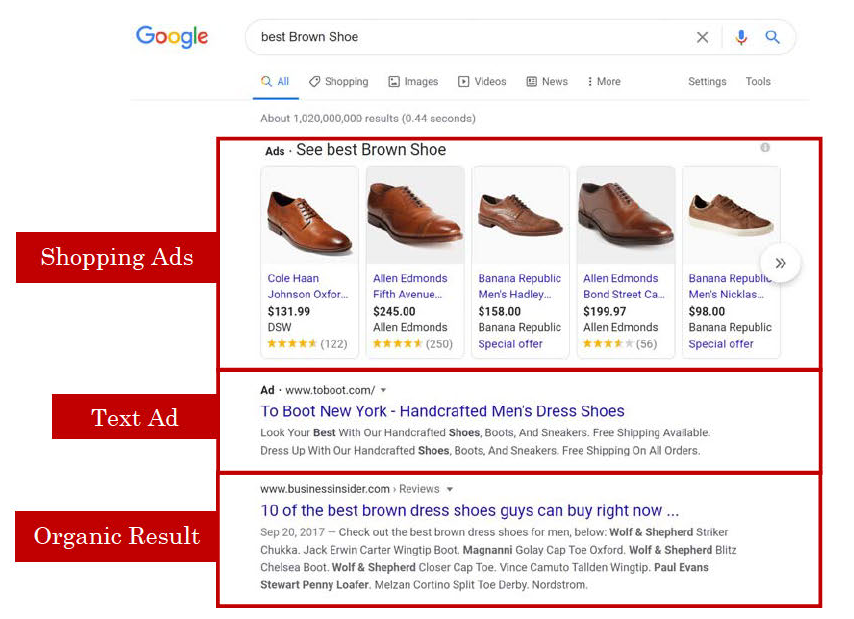
\includegraphics{US-v-Google-Complaint-figures/fig3.png}
\end{figure}

%%%
%%%
%%%
%%%
%%%
%%%
%%%

% 32.

%%%
Some specialized search providers also sell search ads. For example, advertisers
%%%
can buy specialized search ads for goods sold on Amazon, hotels presented on Expedia, and local
services listed on Yelp.

% 33.

%%%
As the number of users of a general search engine grows, advertisers benefit
%%%
because they want their marketing campaigns to reach large groups of consumers. But users do
not benefit from indirect network effects in an equivalent way. As Google’s Chief Economist has
explained, “users do not decide which search engine to use based on the number of advertisers.”

% 34.

%%%
Today, the search advertising business in the United States is enormous—over
%%%
\$50 billion per year—and dominated by Google. Because of Google’s user base and scale, the
company’s search ads have become a “must have” for many advertisers. Advertising agencies
and larger companies often have entire groups that manage search advertising, mostly focused on
Google.

% B.
\subsection{Importance of Scale}
%%%

% 35.

%%%
Scale is of critical importance to competition among general search engines for
%%%
consumers and search advertisers. Google has long recognized that without adequate scale its
rivals cannot compete. Greater scale improves the quality of a general search engine’s
algorithms, expands the audience reach of a search advertising business, and generates greater
revenue and profits.

% 36.

%%%
The additional data from scale allows improved automated learning for algorithms
%%%
to deliver more relevant results, particularly on `fresh' queries (queries seeking recent
information), location-based queries (queries asking about something in the searcher's vicinity),
and `long-tail' queries (queries used infrequently).

% 37.

%%%
Scale is also important for search advertising because advertisers pay more to buy
%%%
ads from a search provider with a large audience of potentially interested customers. Google can
%%%
%%%
%%%
%%%
deliver enormous audiences, especially in mobile, which its competitors cannot. Google’s scale
also enables it to better discern which ads are most relevant for which queries.

% 38.

%%%
Further, to recoup the large investment in creating and maintaining a general
%%%
search engine, scale is critical to generating the necessary revenues and profits. Even a
competitor that syndicates its search results from other general search engines must make
substantial investments to compete. The most effective way to achieve scale is for the general
search engine to be the preset default on mobile devices, computers, and other devices, as
described in more detail below.

%%% C.
\subsection{
%%%
General Search Engine Distribution and Default Status}
%%%

% 39.

%%%
Search is like many other businesses in that the owners of general search engines
%%%
can benefit greatly from a network of distributors to get their products to consumers. Distribution
of general search engines takes place primarily through search access points, such as browsers
and search apps, typically located on mobile devices and computers. More recently, searches
have become available on IoT devices.

% 40.

%%%
General search service providers can enter into agreements with various
%%%
distributors, including computer and mobile-device manufacturers, cell phone carriers, and
browser developers, to secure preset default status on computer and mobile-device search access
points.

% 41.

%%%
New computers and new mobile devices generally come with a number of
%%%
preinstalled apps and out-of-the-box settings. Computers and mobile devices generally have apps
preinstalled that include search access points, such as browsers, search apps and widgets, and
voice assistants. Mobile devices may also have hardware features—such as a home button
triggering a voice assistant—that a consumer can use to invoke apps with search functionality.
Each of these search access points can and almost always does have a preset default general
%%%
%%%
%%%
%%%
search engine. Being the preset default general search engine is particularly valuable because
consumers rarely change the preset default.

% 1.


% 42.

%%%
\subsubsection{The Mobile Search Distribution Channel}
%%%
With roughly 60~percent of searches, mobile devices represent the largest and,
%%%
over the last five years, fastest growing search distribution channel.

% 43.

%%%
In the United States, Apple iOS devices—those running on Apple’s proprietary
%%%
mobile operating system—account for roughly 60~percent of mobile-device usage. Apple’s iOS
is a closed ecosystem; Apple does not license iOS to third-party mobile-device manufacturers.
Another roughly 40~percent of mobile-device usage comes from devices that use Android, an
open-source mobile operating system controlled by Google. Unlike iOS, Android is licensable,
which means third-party mobile-device manufacturers can use it as the operating system for their
devices. All other mobile operating systems, combined, account for less than one percent of
mobile-device usage in the United States.

% 44.

%%%
General search services can be delivered to mobile-device users through a variety
%%%
of search access points, including: (1) a browser, (2) a static search bar (search widget, referred
to in Figure~4 as the QSB or quick search box) on the device’s home screen, (3) a search app,
(4) artificial intelligence software (voice assistants) accessed by a button or voice command and
designed to answer voice-initiated queries, and (5) other apps that link to general search engines,
such as smart keyboards. Figure~4, from a 2018 Google strategy deck, provides a more specific
breakdown of how Google delivers its general search service on Android devices.
%%%
%%%
%%%
%%%
%%%
\begin{figure}
\centering
\caption{}
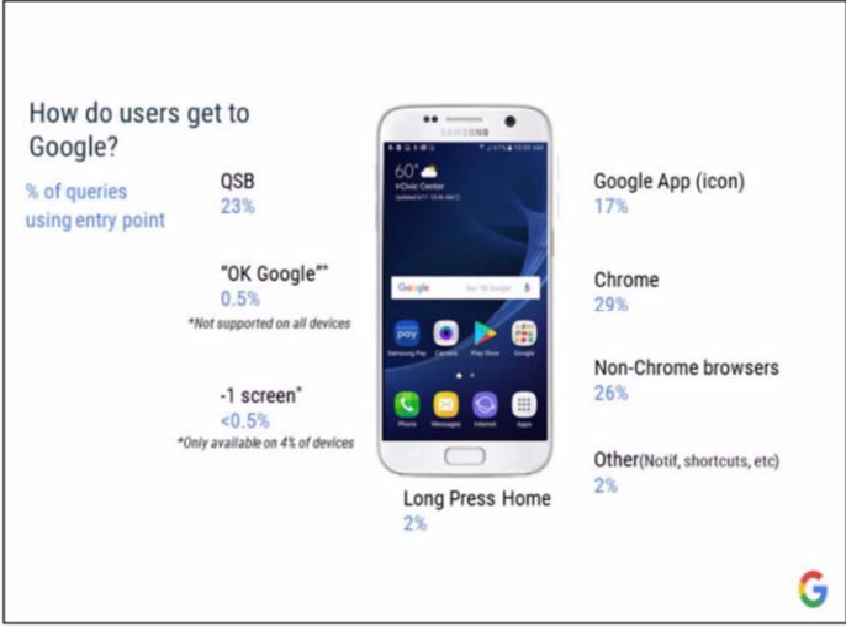
\includegraphics[width=0.7\textwidth]{US-v-Google-Complaint-figures/fig4.png}
\end{figure}
% Figure~4

% 45.

%%%
In the United States, both cell phone carriers and manufacturers sell mobile
%%%
devices. As discussed above, these phones or tablets typically have search access points preset
with a general search engine as the default. These preset defaults are usually governed by a
distribution or licensing agreement. For instance, Google has contracted with Apple for many
years to preset Google’s search engine as the default for Apple’s Safari browser and, more
recently, other search access points on Apple’s mobile devices. When a consumer takes a new
iPhone or iPad out of its box, all the significant access points default to Google as their general
search provider. Indeed, Google has preset default status for an overwhelming share of the search
access points on mobile devices sold in the United States.

% 46.

%%%
For mobile browsers, Google is the default search provider for both Apple Safari
%%%
(approximately 55~percent share) and Google Chrome (over 35~percent share), which together
account for over 90~percent of the browser usage on mobile devices in the United States.
%%%
%%%
%%%
%%%
%%%

% 47.

%%%
Consumers typically do not change their mobile device’s default search functions,
%%%
making securing preset default status for search access points important for effective distribution
of general search engines (and delivery of search ads). As one search competitor noted in 2019,
“For the most part, despite the simplicity of changing a default setting to enable customer choice,
experience shows us that users accept the default search experience that comes with their device
or the browser.” This fact is especially true on mobile devices; as Google observed in a 2018
strategy document, “People are much less likely to change [the] default search engine on
mobile.” Alternative methods of obtaining search access points or encouraging general search
engine usage—such as direct marketing to consumers—are not nearly as effective as
preinstalling search access points on mobile devices and computers.

% 2.


% 48.

%%%
\subsubsection{The Computer Search Distribution Channel}
%%%
When using a computer, most consumers access a general search engine through a
%%%
browser, either by (1) typing a query directly into the address bar at the top of the browser, or
(2) visiting a general search engine web page and entering a query. Many browsers default to a
general-search-engine web page as the home or start screen each time a user activates the
browser; this offers users a convenient way to start their search experience.

% 49.

%%%
In the United States, Google Chrome is the leading computer browser, with
%%%
almost 60~percent market share. Apple’s Safari browser has approximately 16~percent share on
computers. Mozilla’s Firefox has approximately 7~percent share, and Microsoft’s Edge and
Internet Explorer together have approximately 15~percent share. Other small browsers have a
combined share of less than 4~percent. With the exception of Microsoft, most browser developers
have agreed with Google to preset its search engine as the default search provider.
%%%
%%%
%%%
%%%
%%%

% 50.

%%%
Preset default settings are important for computers. Consumers may not
%%%
understand that they can change the browser’s preset default general search engine, or consumers
may not bother to invest the time to make such a switch.

% 51.

%%%
For both mobile and computer search access points, being preset as the default is
%%%
the most effective way for general search engines to reach users, develop scale, and become or
remain competitive.

%%% D.
\subsection{
%%%
Distribution Agreements in Mobile and Computer Channels}
%%%

% 52.

%%%
General search services providers typically enter into licensing and distribution
%%%
agreements with manufacturers and carriers that distribute mobile devices with search access
points. In the United States, roughly 60~percent of all search queries are covered by Google’s
exclusionary agreements. On mobile devices, Google’s exclusionary agreements cover more than
80~percent of all U.S. search queries.

% 53.

%%%
Of the remaining search queries not covered by Google’s exclusionary contracts,
%%%
almost half take place on search access points owned by Google. Google is a vertically integrated
search provider and distributes search in part through several of its own properties, including for
example its browser (Chrome) and phone (Pixel). Between its exclusionary contracts and ownedand-operated properties, Google effectively owns or controls search distribution channels
accounting for roughly 80~percent of the general search queries in the United States.

% 54.

%%%
Google’s distribution agreements come in three basic types, with the specific
%%%
terms of each agreement depending upon the counterparty and the search access points at issue.
First, Google requires Android device manufacturers that want to preinstall Google’s proprietary
apps to sign an anti-forking agreement; these agreements set strict limits on the manufacturers’
ability to sell Android devices that do not comply with Google’s technical and design standards.
%%%
%%%
%%%
%%%
%%%

% 55.

%%%
Next, for Android device manufacturers that sign an anti-forking agreement,
%%%
Google provides access to its vital proprietary apps and application program interfaces (APIs) for
preinstallation, but only if the manufacturers contractually agree to (1) take a bundle of other
Google apps, (2) make certain apps undeletable, and (3) give Google the most valuable and
important real estate on the default home screen.

% 56.

%%%
Finally, Google provides a share of its search advertising revenue to Android
%%%
device manufacturers, mobile phone carriers, competing browsers, and Apple; in exchange,
Google becomes the preset default general search engine for the most important search access
points on a computer or mobile device. As a practical matter, users rarely switch the preset
default general search engine. In many cases, the agreements relating to mobile devices go even
further, expressly prohibiting (1) the preinstallation of any rival general search services, and (2)
the setting of other defaults to rival general search engines. This means that Google is the only
preset default search provider preinstalled on the device.

% 57.

%%%
These agreements work exactly as Google designed them—to foreclose
%%%
distribution to Google’s search rivals, weakening them as competitive alternatives for consumers
and advertisers by denying them scale.

% 1.


% 58.

%%%
\subsubsection{Background on Mobile Strategy and Development of Android Ecosystem}
%%%
Google’s anticompetitive agreements must be understood against the backdrop of
%%%
Google’s overall business strategy. When Google was formed and achieved initial success in the
late 1990s and early 2000s, internet searches were almost exclusively performed through
browsers on computers. But as Google told investors in its 2007 Form 10-K: “More individuals
are using non-desktop devices to access the internet. If users of these devices do not widely
adopt versions of our web search technology, products or operating systems developed for these
devices, our business could be adversely affected.”
%%%
%%%
%%%
%%%

% 59.

%%%
In a mobile world, Google had to deal with mobile device manufacturers (such as
%%%
LG, Motorola, and Samsung), and carriers (such as AT\&T, T-Mobile/Sprint, and Verizon) that
would hold sway over distribution of search and search ads. Google thus asked internally, “How
can we conquer the world’s major wireless markets simultaneously?”

% 60.

%%%
The answer started with Android, a mobile operating system that Google
%%%
purchased in 2005. In 2007, Google released the Android code for free under an open-source
license. Being “open source” means that anyone can access the source code and use it to make
their own, modified operating system—a “fork.” This was key to Android’s adoption.

% 61.

%%%
First, Google’s apparent lack of control over an open-source operating system
%%%
attracted skeptical manufacturers and carriers of mobile phones to use Android instead of the
other choices then available. As the Android team leader observed to Google’s board of
directors, “Google was historically seen as a threat” to these distributors. But an open-source
model suggested that they—and not Google—would ultimately retain control over their devices
and the app ecosystem on those devices.

% 62.

%%%
Second, once enough major distributors agreed to use Android, the operating
%%%
system attracted developers looking for wide distribution of their apps. As more app developers
focused their efforts on designing Android apps, Android became more attractive to consumers,
which in turn led even more developers to design for Android. The result was a must-have
ecosystem of Android apps.

% 63.

%%%
Third, to help the Android ecosystem achieve critical mass and to advance the
%%%
network effects, Google “shared” its search advertising and app store revenues with distributors
as further inducement to give up control. As one senior executive explained about Android
Market, an earlier name for Google’s app store, “Android Market is a bitter pill for carriers, and
%%%
%%%
%%%
%%%
%%%
a generous revenue share is the sugar that makes it go down smoother.” In other words,
beginning over ten years ago, Google used revenue sharing to attract partners to Android; as
discussed below, Google uses revenue sharing to keep them locked in today.

% 64.

%%%
By 2010, the Android team leader noted that “Android is poised for world
%%%
domination—the success story of the decade.” He was right; the strategy worked. The “Google
Play” app store has a massive library of apps, making it essential for Android distributors to have
on their devices. As for the operating system itself, it quickly became the dominant licensable
mobile operating system in the United States. In the four years between 2009 and 2012,
Android’s share of licensable mobile operating systems on smartphones in the United States
more than tripled, reaching about 80~percent. Today, Android represents over 95~percent of
licensable mobile operating systems for smartphones and tablets in the United States and
accounts for over 70~percent of all mobile device usage worldwide. The only other mobile
operating system with significant market share in the United States is Apple’s iOS, which is not
licensable.

% 65.

%%%
Control over Android has always been a critical issue. As Google’s Android team
%%%
leader asked at the time: “How do we retain control of something we gave away?” Google’s
answer is the set of contractual “carrots” and “sticks” discussed below that empower Google to
“[o]wn the ecosystem” and help thwart any alternative mobile ecosystem from developing that
could support a different search provider.
%%%
%%%
%%%
%%%
%%%
% Figure~5
\begin{figure}
\caption{}
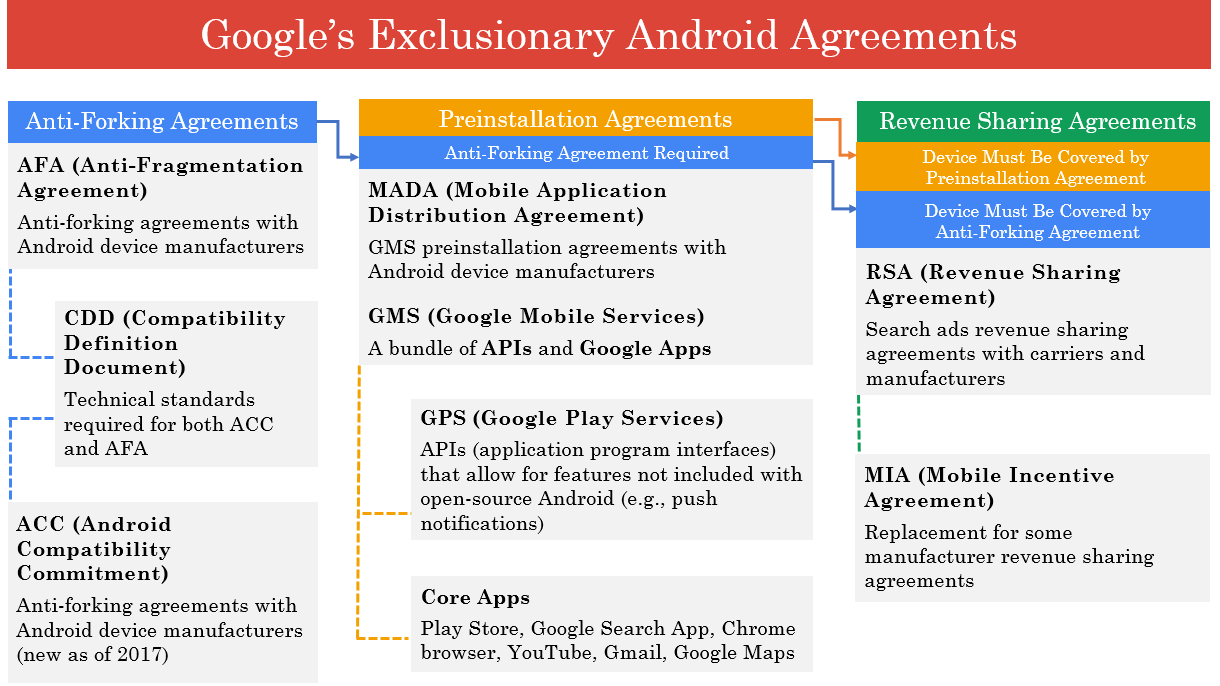
\includegraphics{US-v-Google-Complaint-figures/fig5.png}
\end{figure}

% 2.


% 66.

%%%
\subsubsection{Anti-Fragmentation Agreements and Compatibility Commitments
(Android Mobile Devices)}
%%%
The Android operating system is open source; Google updates the Android code
%%%
periodically and makes it publicly available. But Google takes steps to minimize the risk that a
developer creates an Android fork to compete with the Android ecosystem controlled by Google.
By limiting the existence of devices running Android forks, Google limits possible distribution
channels available to its search rivals.

% 67.

%%%
One way Google retains control of the Android ecosystem is through anti-forking
%%%
agreements. These agreements broadly prohibit manufacturers from taking “any actions that may
cause or result in the fragmentation of Android.” Notably, “fragmentation” is left undefined,
giving Google wide latitude in practice.
%%%
%%%
%%%
%%%
%%%

% 68.

%%%
Google’s anti-forking agreements specifically forbid manufacturers from
%%%
developing or distributing versions of Android that do not comply with Google-controlled
technical standards, as defined in its Android Compatibility Definition Document (CDD).

% 69.

%%%
Two types of anti-forking agreements exist. Before 2017, Google required
%%%
distributors to sign Anti-Fragmentation Agreements (AFAs). In 2017, while being investigated
by the European Commission (and long after Google had locked up its monopoly status), Google
began shifting its anti-forking restrictions from AFAs to new Android Compatibility
Commitments (ACCs). Today, Google has an AFA or ACC with the leading Android device
manufacturers, including LG, Motorola, and Samsung.

% 70.

%%%
ACCs are marginally less onerous than AFAs because they allow manufacturers
%%%
to build devices or components for third parties to sell to consumers, even if those devices or
components do not comply with Google’s technical standards. But ACCs, like AFAs, prohibit
signatories from manufacturing Android forks of their own, distributing devices with Android
forks, or using their powerful brands to market forks on behalf of third parties. Most well-known
Android manufacturers are bound by AFAs or ACCs.

% 71.

%%%
The AFAs and ACCs do not just restrict manufacturers’ ability to build and
%%%
distribute innovative versions of mobile phones. Over time, Google has extended the Android
CDD such that its specifications apply to tablets and emerging technologies such as smart TVs,
watches, and automotive devices. Manufacturers that hope to release Android-based versions of
these products must comply with Google’s standards as well.

% 3.


% 72.

%%%
\subsubsection{Mobile Application Distribution Agreements (Android Mobile Devices)}
%%%
Manufacturers agree to anti-forking agreements in part because they are a
%%%
precondition to receiving a license to distribute devices with must-have proprietary Google apps
and APIs (the set of technical specifications that enable software applications to communicate
%%%
%%%
%%%
%%%
with each other, operating systems, and hardware). This license is provided only through
preinstallation agreements—called Mobile Application Distribution Agreements, or MADAs.
Leading Android device manufacturers, such as LG, Motorola, and Samsung, are MADA
licensees.

% 73.

%%%
Over time, Google has chosen to include important features and functionality in
%%%
Google’s own ecosystem of proprietary apps and APIs, rather than the open-source Android
code. Google refers to this proprietary layer as “Google Mobile Services” (GMS). GMS includes
many popular apps, such as Google’s search app, Chrome, YouTube, and Google Maps. GMS
also includes Google Play, Google’s app store. An app store is one of the most valuable features
of a mobile device because it offers access to compatible apps that do not come preinstalled on
the device. Google Play offers about three million apps, more than any other app store (including
Apple’s App Store, which is compatible only with Apple devices). More than 90~percent of apps
on Android devices are downloaded through Google Play. For years, Google Play has been the
only commercially significant app store option for Android manufacturers.

% 74.

%%%
Another key part of GMS is the set of APIs that allow developers to access certain
%%%
important features. The APIs available within GMS are part of “Google Play Services” (GPS).
GPS allows apps, including third-party apps, to perform functions that are not possible using the
open-source version of Android. For example, using the open-source Android system, third-party
apps cannot provide basic “push notifications,” enable in-app purchases through Google Play, or
use data from Google Maps; to have these functionalities, third-party apps must use GPS.

% 75.

%%%
The integration of key functions with GPS makes it more difficult for third-party
%%%
Android developers to port their apps to Android forks because the apps are designed to interact
%%%
%%%
%%%
%%%
%%%
with Google’s proprietary APIs. And as the functionality gap between open-source Android apps
and Google’s proprietary apps grows, developers are more dependent on GPS.

% 76.

%%%
Signing a preinstallation agreement is the only way for an Android device
%%%
manufacturer to preinstall any Google app, including Google Play. It is also the only way an
Android device manufacturer can gain access to GPS and the APIs many developers need for
their apps to work properly, at least without expensive and time-consuming reprogramming. But
any manufacturer installing Google Play or GPS must preinstall a full suite of apps identified by
Google, including the search access points most frequently used by consumers: Chrome, Google
search app, Google search widget, and Google Assistant. Google’s search engine is the default
on all these search access points. Indeed, Google uses the MADAs to control the appearance of
Android devices, requiring the manufacturer to place the Google search widget on the home
screen, and to preinstall Chrome, the Google search app, and other apps in a way that makes
them undeletable by the user.

% 77.

%%%
Moreover, before 2017, most MADAs also required manufacturers to set Google
%%%
as the default general search engine for all key search access points on any device with
preinstalled Google apps—these requirements are now found in the revenue sharing agreements
discussed below.

% 4.


% 78.

%%%
\subsubsection{Revenue Sharing Agreements (Android Mobile Devices)}
%%%
Google enters into search revenue sharing agreements (RSAs) with Android
%%%
manufacturers and carriers. Google generally requires exclusive distribution as the sole preset
default general search service on an ever-expanding list of search access points; in exchange,
Google remits to these companies a percentage of search advertising revenue. Google offers
revenue share to Android device manufacturers only if they are MADA licensees, and Google
offers revenue share to carriers only for devices built by manufacturers that are MADA
%%%
%%%
%%%
%%%
licensees. The leading U.S. carriers (AT\&T, T-Mobile, and Verizon) and the leading Android
device manufacturer (Samsung) have RSAs with Google.

% 79.

%%%
Some of Google’s revenue sharing agreements require blanket coverage for all
%%%
Android devices sold by Google’s counterparty. Under this version of the revenue sharing
agreements, the distributor receives a payment from Google only if all the distributor’s Android
devices comply with the exclusivity requirements. Other revenue sharing agreements provide for
a model-by-model choice. Under this version of the agreements, for the distributor to receive a
cut of the advertising revenue from any units of a model, every unit of that model must comply
with the exclusivity requirements.

% 80.

%%%
As innovation has increased the number of search access points on mobile
%%%
devices—including smart keyboards and voice assistants—Google has expanded its RSAs to
close off these avenues to search rivals.

% 5.


% 81.

%%%
\subsubsection{Mobile Incentive Agreements (Android Mobile Devices)}
%%%
In Google’s latest round of negotiations with some Android manufacturers,
%%%
Google has replaced RSAs with mobile incentive agreements (MIAs), under which Google pays
manufacturers to (1) forego preinstalling rival general search services on their Android devices
and (2) comply with a significant number of “incentive implementation requirements”—
including preloading up to fourteen additional Google apps. LG and Motorola have MIAs with
Google.

% 82.

%%%
To maximize payments under the MIAs, the manufacturers must also set Google
%%%
as the default for all search access points on nearly all of their devices. Moreover, Google
generally retains “sole discretion” to determine what constitutes a “search access point,” and thus
controls the coverage of its exclusive contracts. Although the MIAs change the payment
%%%
%%%
%%%
%%%
%%%
structure for certain manufacturers, the agreements achieve the same end as their predecessors:
search exclusivity for Google.

% 83.

%%%
Today, Google has revenue sharing agreements (RSAs or MIAs) with all major
%%%
U.S. carriers and Android device manufacturers, as well as a number of smaller carriers and
manufacturers. Google’s revenue sharing agreements (and preinstallation agreements) with
Android device manufacturers, together, account for more than 30~percent of mobile device
usage in the United States.

% 6.


% 84.

%%%
\subsubsection{Revenue Sharing Agreements (Apple and Others)}
%%%
Google’s revenue sharing agreements are not limited to its Android partners.
%%%
Google has entered into revenue sharing agreements with rival browsers and other device
manufacturers, further blocking off search access points from competition.

% 85.

%%%
Most significantly, Google has had a series of search distribution agreements with
%%%
Apple, effectively locking up one of the most significant distribution channels for general search
engines. Apple operates a tightly controlled ecosystem and produces both the hardware and the
operating system for its popular products. Apple does not license its operating systems to thirdparty manufacturers and controls preinstallation of all apps on its products. The Safari browser is
the preinstalled default browser on Apple computer and mobile devices. Apple devices account
for roughly 60~percent of mobile device usage in the United States. Apple’s Mac OS accounts for
approximately 25~percent of the computer usage in the United States.

% 86.

%%%
In 2005, Apple began using Google as the preset default general search engine for
%%%
Apple’s Safari browser. In return, Google gave Apple a significant percentage of Google’s
advertising revenue derived from the search queries on Apple devices. Two years later, Google
extended this agreement to cover Apple’s iPhones. In 2016, the agreement expanded further to
cover additional search access points—Siri (Apple’s voice-activated assistant) and Spotlight
%%%
%%%
%%%
%%%
(Apple’s system-wide search feature)—making Google the preset default general search engine
for both services. Today, Google’s distribution agreement with Apple gives Google the coveted,
preset default position on all significant search access points for Apple computers and mobile
devices.

% 87.

%%%
Today, Google has RSAs with nearly every significant, non-Google browser other
%%%
than those distributed by Microsoft, including Mozilla’s Firefox, Opera, and UCWeb. These
agreements generally require the browsers to make Google the preset default general search
engine for each search access point on both their web and mobile versions.

% \section{III. \textsc{General markets}}

\section{\rmfamily\textsc{Relevant Markets}}

\subsection{General Search Services in the United States}

% 1.

%%%

% 88.

%%%

%%%
\subsubsection{General Search Services in the United States Is a Relevant Antitrust
Market}
%%%
General search services in the United States is a relevant antitrust market. General
%%%
search services allow consumers to find responsive information on the internet by entering
keyword queries in a general search engine such as Google, Bing, or DuckDuckGo.

% 89.

%%%
General search services are unique because they offer consumers the convenience
%%%
of a “one-stop shop” to access an extremely large and diverse volume of information across the
internet. Consumers use general search services to perform several types of searches, including
navigational queries (seeking a specific website), informational queries (seeking knowledge or
answers to questions), and commercial queries (seeking to make a purchase).

% 90.

%%%
Other search tools, platforms, and sources of information are not reasonable
%%%
substitutes for general search services. Offline and online resources, such as books, publisher
websites, social media platforms, and specialized search providers such as Amazon, Expedia, or
Yelp, do not offer consumers the same breadth of information or convenience. These resources
%%%
%%%
%%%
%%%
%%%
are not “one-stop shops” and cannot respond to all types of consumer queries, particularly
navigational queries. Few consumers would find alternative sources a suitable substitute for
general search services. Thus, there are no reasonable substitutes for general search services, and
a general search service monopolist would be able to maintain quality below the level that would
prevail in a competitive market.

% 91.

%%%
The United States is a relevant geographic market for general search services.
%%%
Google offers users in the United States a local domain website with search results optimized
based on the user’s location in the United States. General search services available in other
countries are not reasonable substitutes for general search services offered in the United States.
Google analyzes search market shares by country, including the United States. Therefore, the
United States is a relevant geographic market.

% 2.


% 92.

%%%
\subsubsection{Google Has Monopoly Power in the General Search Services Market in
the United States}
%%%
Google has monopoly power in the United States general search services market.
%%%
There are currently only four meaningful general search providers in this market: Google, Bing,
Yahoo!, and DuckDuckGo. According to public data sources, Google today dominates the
market with approximately 88~percent market share, followed far behind by Bing with about
seven percent, Yahoo! with less than four percent, and DuckDuckGo with less than two percent.
%%%
%%%
%%%
%%%
%%%
\begin{figure}
\caption{}
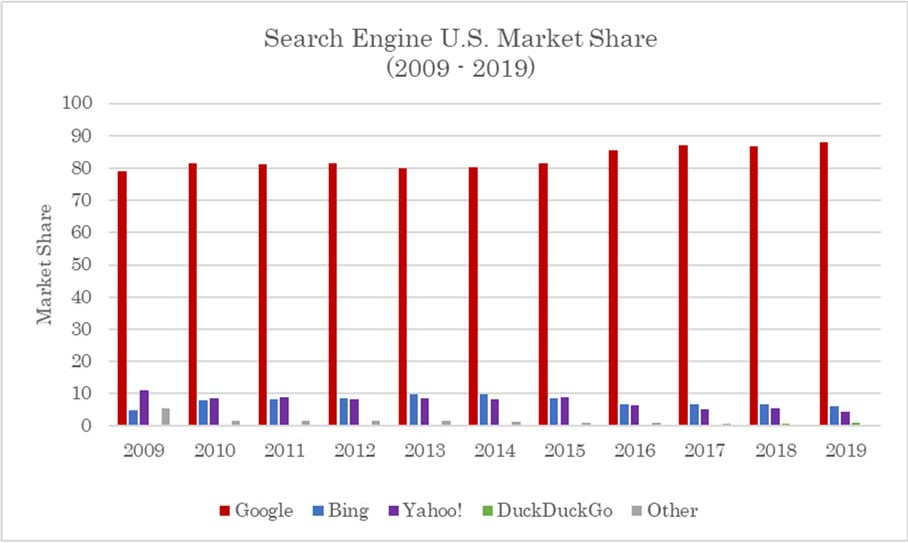
\includegraphics{US-v-Google-Complaint-figures/fig6.png}
\end{figure}
% Figure~6

% 93.

%%%
Over the years, Google has steadily increased its dominant position in general
%%%
search services. In July 2007, Google estimated its general search services market share at
68~percent. By June 2013, Google estimated that its share in the United States had already
increased to 77~percent on computers. By April 2018, Google estimated that its share was
79~percent on computers and 93.5~percent on mobile. More recently, Google has accounted for
almost 90~percent of all general search engine queries in the United States, and almost 95~percent
of queries on mobile devices. Recent share estimates are in Figures 7 and 8.
%%%
%%%
%%%
%%%
%%%
% Figure~7

% % 94.

% %%%
% Figure~8
\begin{figure}
\caption*{\textbf{Figure 7\qquad Figure 8}}
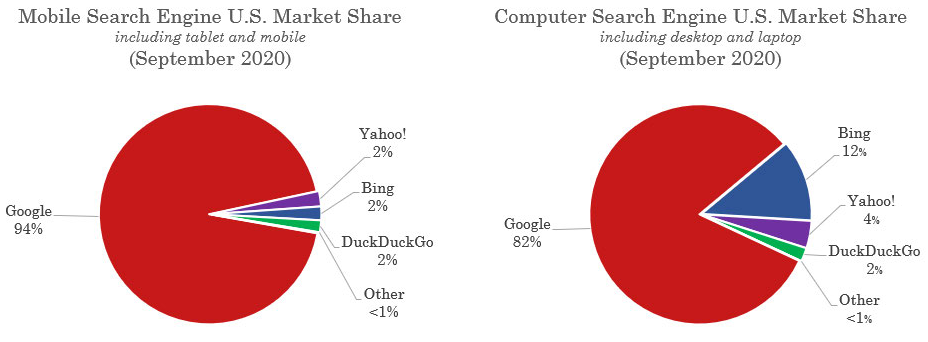
\includegraphics{US-v-Google-Complaint-figures/fig7.png}
\end{figure}

%%%
There are significant barriers to entry in general search services. The creation,
%%%
maintenance, and growth of a general search engine requires a significant capital investment,
highly complex technology, access to effective distribution, and adequate scale. For that reason,
only two U.S. firms—Google and Microsoft—maintain a comprehensive search index, which is
just a single, albeit fundamental, component of a general search engine.

% 95.

%%%
Scale is also a significant barrier to entry. Scale affects a general search engine’s
%%%
ability to deliver a quality search experience. The scale needed to successfully compete today is
greater than ever. Google’s anticompetitive conduct effectively eliminates rivals’ ability to build
the scale necessary to compete.

% 96.

%%%
Google’s large and durable market share and the significant barriers to entry in
%%%
general search services demonstrate Google’s monopoly power in the United States.
%%%
\subsection{B. Search Advertising in the United States and General Search Text Advertising in
the United States Are Relevant Antitrust Markets}

% 1.

%%%

% 97.

%%%
\subsubsection{Search Advertising Is a Relevant Product Market}
%%%
Search advertising in the United States is a relevant antitrust market. The search
%%%
advertising market consists of all types of ads generated in response to online search queries,
including general search text ads (offered by general search engines such as Google and Bing)
%%%
%%%
%%%
%%%
and other, specialized search ads (offered by general search engines and specialized search
providers such as Amazon, Expedia, or Yelp).

% 98.

%%%
Search ads enable advertisers to target marketing messages in real time in
%%%
response to queries entered by a consumer. Thus, a user’s general search query has the important
function to an advertiser of revealing the searcher’s intent. The ability of search ads to respond to
consumer inquiries, at the moment the consumer is investigating a subject relevant to an
advertiser’s product or service, makes these ads highly valuable to advertisers and distinguishes
them from other types of advertising that cannot be similarly targeted, whether online or offline.

% 99.

%%%
Other forms of advertising are not reasonably substitutable for search ads. For
%%%
example, “offline” ads such as newspaper, billboard, TV, and radio ads cannot be targeted at a
specific consumer based on the consumer’s real-time, self-disclosed interests. Similarly, other
forms of online ads, such as display ads or social media ads, do not enable advertisers to target
customers based on specific queries and are generally aimed at consumers who are further from
the point of purchase. As Google’s Chief Economist explained: “One way to think about the
difference between search and display/brand advertising is to say that ‘search ads help satisfy
demand’ while ‘brand advertising helps to create demand,’” and “[d]isplay and search
advertising are complementary tools, not competing ones.”

% 100.

%%%
Few advertisers would find alternative sources a suitable substitute for search
%%%
advertising. Thus, there are no reasonable substitutes for search advertising, and a search
advertising monopolist would be able to maintain prices above the level that would prevail in a
competitive market.

% 2.


% 101.

%%%
\subsubsection{General Search Text Advertising Is a Relevant Product Market}
%%%
There also is a relevant product market for general search text advertising that is
%%%
wholly contained within the broader search advertising market. General search text ads are sold
%%%
%%%
%%%
%%%
by general search engines, typically placed just above or below the organic search results on a
SERP, and resemble the organic results that appear on a general search engine’s SERP, with a
subtle notation that they are “ads” or “sponsored.” In contrast, other types of search 
ads---specifically, specialized search ads---typically are visually different from general search text ads
and convey different types of information. For example, a Google Shopping Ad normally
includes an image of the product, its price, and star-based ratings (see Figure~3). In 2018, general
search text ads accounted for close to 85~percent of Google’s search ad revenue.

% 102.

%%%
General search text ads are distinct from specialized search ads in ways that limit
%%%
their substitutability for most purposes, including their scope of coverage, purpose, format, and
sales process. Indeed, for many advertisers that purchase general search text ads, there are no
reasonable alternatives for these ads, which renders these advertisers particularly vulnerable to
targeted price increases. General search text ads on Google are vitally important for many
different types of advertisers, including companies that prefer to sell directly to consumers from
their own websites and companies that want to protect their brand names on Google.

% 103.

%%%
General search text ads can be delivered in response to search queries related to
%%%
any subject that users explore on the internet. General search text ads are offered predominantly
by the two companies that operate general search engines: Google and Microsoft (Bing); Bing
also syndicates general search text ads for Yahoo! and DuckDuckGo. By contrast, other kinds of
search ads are provided by specialized search providers in response to narrower and deeper
searches in their areas of specialization, such as retail (e.g., Amazon), travel (e.g., Kayak), or
local (e.g., Yelp).

% 104.

%%%
General search text ads often target consumers further from an actual sale or
%%%
“conversion” than specialized search ads. Users often rely on a general search engine such as
%%%
%%%
%%%
%%%
%%%
Google to start a search of the entire web to explore an interest, consider options, and form a
preference, often about a purchase. An advertiser often will buy a general search text ad to drive
these searchers down the purchase funnel to the advertiser’s website to shop for a product or
service. In part for this reason, specialized search providers, such as Amazon, Expedia, and
eBay, are among Google’s largest customers for general search text ads—i.e., they buy general
search text ads to drive consumers to their specialized search sites, where they then sell
specialized search ads to advertisers who want to reach those interested consumers at or near the
point of purchase. Because general search text ads and specialized ads serve different functions,
advertisers often view these ads as complements.

% 105.

%%%
General search text ads link to the advertiser’s website, so the user can “click out”
%%%
to that site. By contrast, ads by specialized search providers often link to webpages on that
specialized search provider’s own website. For example, if a company sells a product on
Amazon and buys an ad on Amazon to promote its product, the ad links to the Amazon page on
which the advertised product can be purchased—not the seller’s own website. This kind of
search ad is called a “click in” ad. Thus, general search text ads can be purchased by advertisers
that do not sell their products or services on specialized search sites (such as Amazon) as well as
advertisers that prefer to sell their products or services directly to consumers.

% 106.

%%%
Few general search text advertisers would find alternative sources a suitable
%%%
substitute for general search text advertising. Thus, there are no reasonable substitutes for
general search text advertising, and a general search text advertising monopolist would be able to
maintain prices above the level that would prevail in a competitive market.

% 3.


% 107.

%%%
The United States Is a Relevant Geographic Market
%%%
The United States is a relevant geographic market for both the search advertising
%%%
and the general search text advertising markets. Market participants recognize this in the
%%%
%%%
%%%
%%%
ordinary course of business. For example, Google offers advertisers the ability to target and
deliver ads based on the location of consumers in the United States, and Google search is
customized for particular countries. Google also separately tracks revenue for the United States.

% 4.


% 108.

%%%
Google Has Monopoly Power in the Search Advertising and General
Search Text Advertising Markets in the United States
%%%
Google has monopoly power in the search advertising market. Based on public
%%%
estimates of total search advertising spending in the United States, Google’s share of the U.S.
search advertising market is over 70~percent. This market share understates Google’s market
power in search advertising because many search-advertising competitors offer only specialized
search ads and thus compete with Google only in a limited portion of the market.

% 109.

%%%
Google also has monopoly power in the general search text advertising market.
%%%
Google’s market share of the U.S. general search text advertising market also exceeds
70~percent. Google’s share of the general search text advertising market well exceeds its share of
the search advertising market.

% 110.

%%%
There are barriers to entry in these advertising markets that protect Google’s
%%%
advertising monopolies. Most critically, search advertising of any kind requires a search engine
with sufficient scale to make advertising an efficient proposition for businesses. Specialized
search engines require significant investment, including the cost of populating and indexing
relevant data, distribution, developing and maintaining a search algorithm, and attracting users.
Search advertising of any kind also requires (1) a user interface through which advertisers can
buy ads, (2) software to facilitate the sales process, and (3) a sales and technical support staff.
The same barriers to entry that apply to general search services also protect Google’s general
search text advertising monopoly.
%%%
%%%
%%%
%%%
%%%
% V.

% 111.

%%%
\section{\textsc{Anticompetitive Conduct}}
%%%
Google is a monopolist in the general search services, search advertising, and
%%%
general search text advertising markets. Google aggressively uses its monopoly positions, and
the money that flows from them, to continuously foreclose rivals and protect its monopolies.

% 112.

%%%
Google has unlawfully maintained its monopolies by implementing and enforcing
%%%
a series of exclusionary agreements with distributors over at least the last decade. Particularly
when taken together, Google’s exclusionary agreements have denied rivals access to the most
important distribution channels. In fact, Google’s exclusionary contracts cover almost 60~percent
of U.S. search queries. Almost half the remaining searches are funneled through properties
owned and operated directly by Google. As a result, the large majority of searches are covered
by Google’s exclusionary contracts and own properties, leaving only a small fraction for
competitors.

% 113.

%%%
Google’s continued use of the exclusionary agreements over many years, long
%%%
after there was any real competition in general search, has denied its rivals access to the scale
that would allow rivals to increase quality. By depriving them of scale, Google also hinders its
rivals’ ability to secure distribution going forward, insulating Google from competition.

% 114.

%%%
Google’s exclusionary motives influence its negotiations with distributors. Some
%%%
of these exclusionary agreements have been described by Google as an “[i]nsurance policy that
preserves our search and assistant usage.” To preserve its dominance, Google has developed
economic models to measure the “defensive value” of foreclosing search rivals from effective
distribution, search access points, and ultimately competition. Google recognized it could pay
search distributors to “protect [its] market share from erosion.” Google continues to focus on the
exclusionary defensive value of its distribution contracts as it tries to expand its search
dominance into new distribution channels, such as smart home speakers. Here, Google’s
%%%
%%%
%%%
%%%
defensive value “is attributable to protecting access to Search and other Google services that may
otherwise be blocked in a given household” if a user chooses a rival.

% 115.

%%%
In sum, Google deprives rivals of the quality, reach, and financial position
%%%
necessary to mount any meaningful competition to Google’s longstanding monopolies. By
foreclosing competition from rivals, Google harms consumers and advertisers.

%%A.
%%%
\subsection{Google's Agreements Lock Up Mobile Distribution of Search}
%%%

% 116.

%%%
Launched in the infancy of mobile smartphones, Google’s strategy to ward off
%%%
competition for mobile search distribution had two parts. First, Google expanded its existing
search deal with Apple to cover mobile. Second, for other mobile distributors, Google offered its
Android operating system for “free” but with a series of interlocking distribution agreements to
ensure it search-engine dominance in the Android ecosystem.

% 117.

%%%
Google’s strategy worked. Google has almost completely shut out its competitors
%%%
from mobile distribution. As one executive for a competing search product recognized in
frustration last year: “Google essentially [has] locked up ALL DISTRIBUTION” with its Apple
deal and restrictive Android licensing terms, leaving the competitor’s product with “no mobile
volume.”

% 1.


% 118.

%%%
\subsubsection{Distribution on Apple iOS Devices}
%%%
Apple has not developed and does not offer its own general search engine. Under
%%%
the current agreement between Apple and Google, which has a multi-year term, Apple must
make Google’s search engine the default for Safari, and use Google for Siri and Spotlight in
response to general search queries. In exchange for this privileged access to Apple’s massive
consumer base, Google pays Apple billions of dollars in advertising revenue each year, with
public estimates ranging around \$8–12 billion. The revenues Google shares with Apple make up
approximately 15–20~percent of Apple’s worldwide net income.
%%%
%%%
%%%
%%%

% 119.

%%%
Although it is possible to change the search default on Safari from Google to a
%%%
competing general search engine, few people do, making Google the de facto exclusive general
search engine. That is why Google pays Apple billions on a yearly basis for default status.
Indeed, Google’s documents recognize that “Safari default is a significant revenue channel” and
that losing the deal would fundamentally harm Google’s bottom line. Thus, Google views the
prospect of losing default status on Apple devices as a “Code Red” scenario. In short, Google
pays Apple billions to be the default search provider, in part, because Google knows the
agreement increases the company’s valuable scale; this simultaneously denies that scale to rivals.

% 120.

%%%
Apple’s RSA incentivizes Apple to push more and more search traffic to Google
%%%
and accommodate Google’s strategy of denying scale to rivals. For example, in 2018, Apple’s
and Google’s CEOs met to discuss how the companies could work together to drive search
revenue growth. After the 2018 meeting, a senior Apple employee wrote to a Google
counterpart: “Our vision is that we work as if we are one company.”

% 121.

%%%
The current version of the Google-Apple agreement substantially forecloses
%%%
Google's search rivals from an important distribution channel for a significant, multi-year term.
This agreement covers roughly 36~percent of all general search queries in the United States,
including mobile devices and computers. Google estimates that, in 2019, almost 50~percent of its
search traffic originated on Apple devices.

% 122.

%%%
Particularly when considered with the other exclusionary distribution agreements
%%%
discussed below, Google’s hold on Apple’s distribution channel is self-reinforcing, impairing
rival general search engines’ ability to offer competitive products and making Google’s
monopolies impenetrable to competitive discipline. By paying Apple a portion of the monopoly
rents extracted from advertisers, Google has aligned Apple’s financial incentives with its own
%%%
%%%
%%%
%%%
%%%
and set the price of bidding for distribution extraordinarily high—in the billions. And, even if a
rival was willing to make no money from a distribution relationship or could afford to lose
money indefinitely, the rival would likely still fall short because the existing distribution
agreements have for more than a decade denied rivals the benefits of scale, thus limiting (1) the
quality of their general search and search advertising products, as well as (2) the audience to
attract advertisers. In other words, because of the longtime deprivation of scale, no other search
engine can offer Apple (or any other partner) the mix of quality, brand recognition, and
economics that market-dominant Google can.

% 2.


% 123.

%%%
Distribution on Android Devices
%%%
Google controls the Android mobile distribution channel with its distributor
%%%
agreements and owned-and-operated distribution properties.

% 124.

%%%
Even though Android is open source, Google has used Android to protect
%%%
Google’s lucrative general search and search advertising monopolies. Google sets the rules
through anti-forking agreements, preinstallation agreements, and revenue sharing agreements.
Notably, each of these agreements builds on the others to preserve control. Thus, Google will not
pay a revenue share or financial incentive payment on a mobile device unless it is covered by
(1) an anti-forking agreement, (2) a preinstallation agreement ensuring that Google’s search
access points are preinstalled and given prominent placement, and (3) a revenue sharing or
mobile incentive agreement that entitles Google to preset default status and, in most cases,
prohibits preinstallation of search access points with rival general search providers.

% 125.

%%%
Through these interlocking, anticompetitive agreements, Google insulates and
%%%
protects its monopoly profits. One internal Google analysis of these restrictive agreements
concluded that only one percent of Google’s worldwide Android search revenue was currently at
%%%
%%%
%%%
%%%
%%%
risk to competitors. This analysis noted that the growth in Google’s search advertising revenue
from Android distribution was “driven by increased platform protection efforts and agreements.”

\begin{enumerate}
% a)

% 126.

%%%
\item \textit{Anti-Forking Agreements}\quad
%%%
An alternative operating system could serve as a pathway for distribution of
%%%
general search services other than Google. However, Google’s anti-forking agreements inhibit
the development of an operating system based on an Android fork that could serve as a viable
path to market for a search competitor.

% 127.

%%%
Developing an operating system from scratch is extremely expensive, but a
%%%
manufacturer could start with existing Android open-source code for a fraction of the cost.
Moreover, the costs to app developers of “porting” GMS-compatible Android apps to an Android
fork are substantially less than developing apps for an entirely new operating system.

% 128.

%%%
Google’s anti-forking agreements, however, have inhibited operating system
%%%
innovation through forking, ensuring that manufacturers and distributors are beholden to
Google’s version of Android. Distributors know that any violation of an anti-forking agreement
could mean excommunication from Google’s Android ecosystem, loss of access to Google’s
must-have GPS and Google Play, and millions or even billions of dollars in lost revenue sharing.
Thus, distributors avoid anything that Google might deem “fragmentation”—a term that Google
“purposely leave[s] . . . very vague” and interprets broadly.

% 129.

%%%
Pursuant to the preinstallation agreements discussed below, Google also has final
%%%
say over whether a device is found to be compatible with the technical specifications Google
requires manufacturers to meet before they can preinstall GMS. As a Google engineer noted, it
must be “obvious to the [manufacturers] that we are using compatibility as a club to make them
do things we want.” Google views its anti-fragmentation mandate, and its final approval of
%%%
%%%
%%%
%%%
%%%
devices before they launch, as a “poison pill” to prevent deviation from the Google-controlled
Android ecosystem.

% 130.

%%%
Google’s broad interpretation of the anti-forking agreements, and the reluctance it
%%%
creates among Android distributors to support alternative versions of Android, presents barriers
to entry. These were on display when Amazon developed its Fire OS operating system, a
competing fork of Android. Rather than preinstall Google’s search engine, GPS, Google Play, or
other Google apps on Fire devices, Amazon preinstalled its own proprietary apps and agreed to
make Microsoft’s Bing the preset default general search engine. Amazon originally sold only
Fire OS tablets, but in 2014 it launched a phone that ran on Fire OS. The phone was not a
commercial success and Amazon quickly exited the phone business. Amazon continues to sell
Fire tablets, which account for less than two percent of mobile device usage in the United States.

% 131.

%%%
Google’s anti-forking provisions and policies limited the growth of Amazon’s
%%%
mobile phone, and of Fire OS, because major manufacturers declined to support Amazon’s
phone out of fear doing so would risk their lucrative deals with Google. Manufacturers willing to
work with Amazon did not have the same marketing and logistics capabilities as top
manufacturers. Despite hundreds of millions of dollars in investment over nearly ten years across
tablets and phones, Fire OS still has not reached sufficient critical mass to challenge Google’s
version of Android and provide a significant alternative path to market for search rivals.

% 132.

%%%
No Android fork has made significant inroads to challenge Google for mobile
%%%
devices, and there is no meaningful operating system alternative for manufacturers and carriers
to license. These manufacturers and carriers are beholden to Google’s Android ecosystem, which
Google uses to preserve its monopolies in general search, search advertising, and general search
text advertising. Google’s anti-forking agreements further inhibit the development of alternative
%%%
%%%
%%%
%%%
%%%
Android operating systems for the next generation of search distribution channels, such as smart
watches, smart speakers, smart TVs, and connected automobiles.
b)

% 133.

%%%
\item \textit{Preinstallation Agreements}\quad
Google uses preinstallation agreements -- MADAs -- to ensure that its entire suite
of search-related products is given premium placement on Android GMS devices. Consumers
naturally and regularly turn to these prominently placed search access points to conduct searches.
Preinstallation agreements also reinforce Google's anti-forking requirements, either by including
an anti-forking clause of their own or, more commonly, requiring device manufacturers to be
signatories to an anti-forking agreement.

% 134.

%%%
If a manufacturer wants even one of Google’s key apps and APIs, the device must
%%%
be preloaded with a bundle of other Google apps selected by Google. The six “core” apps are
Google Play, Chrome, Google’s search app, Gmail, Maps, and YouTube. Manufacturers must
preinstall the core apps in a manner that prevents the consumer from deleting them, regardless of
whether the consumer wants them. These preinstallation agreements cover almost all Android
devices sold in the United States.

% 135.

%%%
Google’s preinstallation agreements effectuate a tie, that is, they condition the
%%%
distribution of Google Play and GPS to the distribution of these other apps. This tie reinforces
Google’s monopolies. The preinstallation agreements provide Android device manufacturers an
all-or-nothing choice: if a manufacturer wants Google Play or GPS, then the manufacturer must
also preinstall, and in some cases give premium placement to, an entire suite of Google apps,
including Google’s search products. The forced preinstallation of Google’s apps deters
manufacturers from preinstalling those of competitors. This forecloses distribution opportunities
to rival general search engines, protecting Google’s monopolies.
%%%
%%%
%%%
%%%
%%%

% 136.

%%%
Google recognizes it could “make [the] phone experience better for user[s] by
%%%
ensuring . . . preloaded apps are deletable.” In large part, this is because “[u]sers can free up
space by deleting apps they don’t want.” Consumers desiring to use non-Google search access
points thus suffer because they cannot save storage space on their devices by deleting unwanted
Google apps. In this way, manufacturers must agree to make their phones less attractive to
consumers to accommodate Google’s efforts to lock up search distribution.

% 137.

%%%
Once the manufacturer adopts the necessary suite of Google apps, the search
%%%
access points of those apps are preset to default to Google’s search engine. For example, the
preinstalled version of Chrome is preset to default to Google search. A senior executive at
Google referred to changing Chrome’s preset search default as “totally off the table” and insisted
that if a manufacturer “values their MADA, they cannot modify Chrome’s settings.” The result is
that Google locks up the access points to general search on Android phones, as shown in
Figure~9:
%%%
\begin{figure}
\caption{}
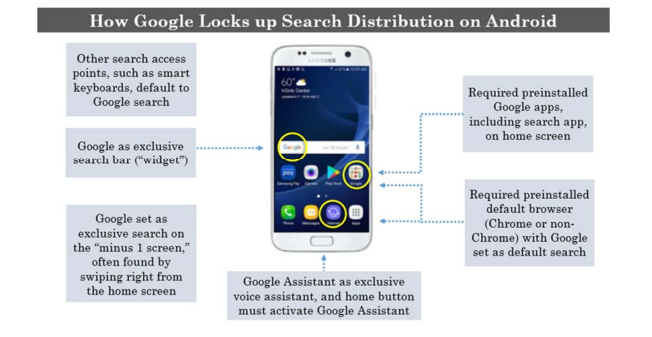
\includegraphics{US-v-Google-Complaint-figures/fig9.PNG}
\end{figure}
%%%
%%%
%%%
%%%
%%%

% 138.

%%%
The preinstallation agreements are even more pernicious than basic ties because
%%%
these agreements force distributors to configure the appearance of their phones to Google’s
specifications. For example, they require manufacturers to put the Google search widget on the
device’s default home screen. Google considers the search widget “an essential part of the
Google brand” and rejects requests by manufacturers to waive the preinstallation agreement’s
search-widget requirement. This locks up another search access point, as it would be impractical
for a manufacturer to preinstall two search widgets on the same home screen.

% 139.

%%%
Google’s preinstallation agreements also impose voice-search preferencing. In
%%%
addition to requiring the preinstallation of Google Assistant, preinstallation agreements require
manufacturers to (1) implement a Google hotword, which activates Google Assistant, and
(2) ensure certain touch actions on the device’s home button directly access Google Assistant or
Google. Google’s agreements with most manufacturers also (3) set Google Assistant as the
default assistant app.

% 140.

%%%
Rivals to Google Assistant are deprived of the same opportunities. Most of
%%%
Google’s preinstallation agreements prevent rival assistants from being the preset default or
using a home button. Google also handicaps rival assistants by limiting the APIs that non-Google
apps can use, ensuring that the useful features, such as “always on” microphone access that
would enable the use of a hotword or the initiation of phone calls, are available only to Google
Assistant. Even Google Assistant’s chief rival—Amazon’s Alexa—is unable to navigate these
disincentives to get significant preinstallation or functional integration on Android devices.

% 141.

%%%
Voice search is an important, emerging access point. Internal Google documents
%%%
have recognized that the “[v]oice platform will become the future of search” and financial
projections for the assistant category recognize “search defensive value.”
%%%
%%%
%%%
%%%
%%%

% 142.

%%%
Partners that depart from the preinstallation agreements risk discipline from
%%%
Google. For example, in 2011, one major electronics manufacturer considered giving a group of
consumers outside the United States a choice between two home screen experiences for their
device: one home screen with the Google search widget and a second home screen with a rival
search widget. Discussing this proposal with colleagues, one Google employee noted “[a]llowing
a mode that does not have Google as the default search provider and completely changes the
home screen” would violate Google’s terms and risk breach.

% 143.

%%%
In 2015, Google was concerned that a major United States carrier would ask
%%%
manufacturers to install a search widget powered by the carrier’s in-house search engine.
Google’s Vice President of Partnerships wrote to a colleague that Google needed to make clear
to manufacturers that “[these] customization requests will not go far” and replacing the Google
search widget with a different search box would violate the preinstallation agreement.
Termination of this default agreement would, in turn, prohibit access to the entire GMS suite,
including Google Play and GPS, and forfeit any potential cut of Google’s search advertising
revenue under a revenue sharing agreement. In short, as the above examples illustrate, Google’s
documents show its efforts to discipline its counterparties, including major electronics companies
and carriers.
%c)

% 144.

%%%
\item \textit{Revenue Sharing Agreements}\quad
%%%
In exchange for a substantial portion of Google’s search advertising revenues,
%%%
Android distributors agree to make Google the preset default general search engine for all
significant search access points on the device. In addition, these agreements typically contain an
exclusivity provision prohibiting the preinstallation of a competing general search service.

% 145.

%%%
Google has recognized for some time that its revenue sharing agreements with
%%%
Android device manufacturers and carriers provide exclusivity for its general search service on
%%%
%%%
%%%
%%%
those devices. As stated explicitly in a draft 2014 Google strategy deck in Figures 10 and 11
below, Google’s revenue sharing arrangements with Android manufacturers or OEMs “provide
exclusivity of Search” and its deals with carriers similarly “prevent[] the pre-installation of other
Search engines or browsers,” thus enabling Google “to protect Search exclusivity on the device
as it makes its way to the user.”
%%%
\begin{figure}
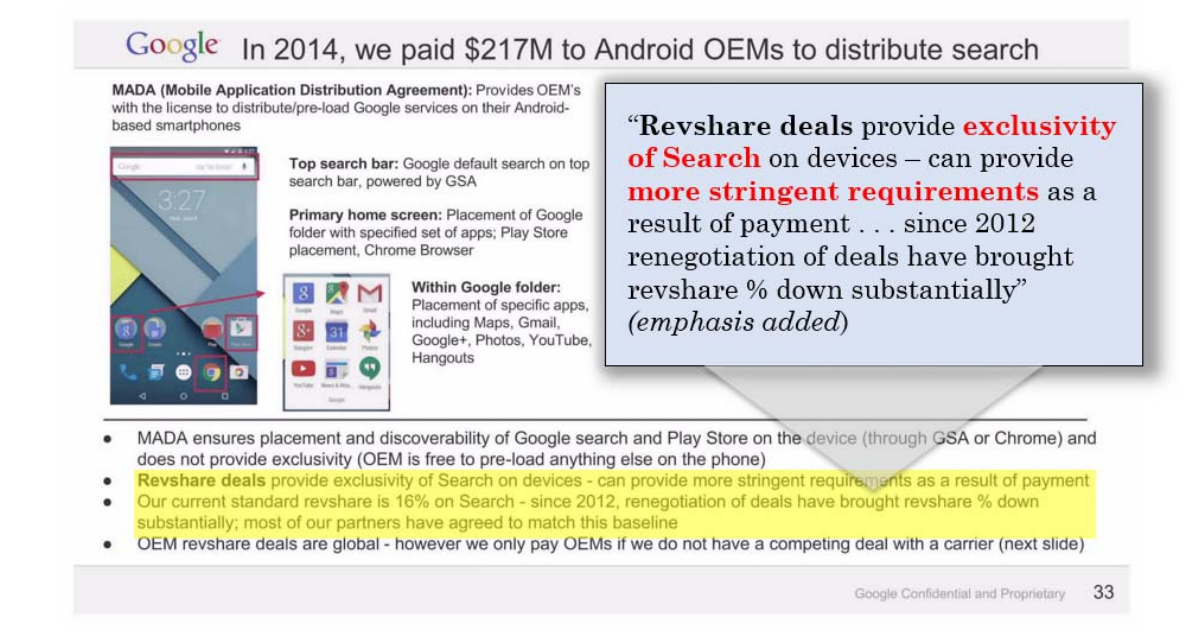
\includegraphics{US-v-Google-Complaint-figures/fig10.PNG}
\caption{(Android manufacturers)}

%%%
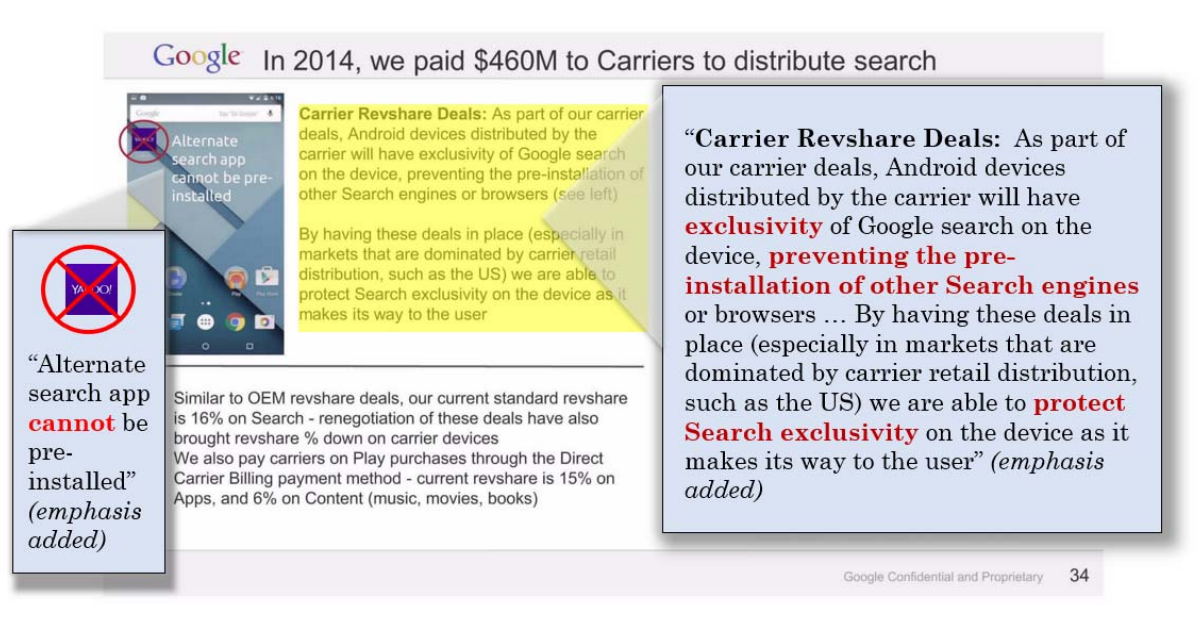
\includegraphics{US-v-Google-Complaint-figures/fig11.PNG}
\caption{(Android carriers)}
\end{figure}
%%%
%%%
%%%
%%%

% 146.

%%%
Similarly, one Google executive acknowledged that exclusivity is “the general
%%%
philosophy of the RSA or one of the tenets of the value exchanged in the RSA.” Another Google
executive noted, “our philosophy is that we are paying revenue share *in return for* exclusivity.”
These agreements are, as that executive further explained, “really important” because “otherwise
Bing or Yahoo can come and steal away our Android search distribution at any time.”

% 147.

%%%
As Google’s documents recognize, the preinstallation agreements and revenue
%%%
sharing agreements work together as a belt-and-suspenders strategy for driving searches to
Google (and therefore away from competitors) on Android devices. As one Google executive
explained in 2017, Google uses revenue sharing agreements “as a lever for motivating partner
behavior that is consistent with our goals for Google and the ecosystem,” and to “drive
incremental revenue (securing search defaults not covered by MADA).” By using its monopoly
profits, Google is able to secure even “more stringent requirements” on manufacturers and
carriers to obtain the preset default position on search access points not covered by the
preinstallation agreements. The combined result of Google’s preinstallation and revenue sharing
agreements is to lock up all the main pathways through which consumers access search on
Android devices, thus foreclosing rivals and protecting Google’s monopoly positions.

% 148.

%%%
The size of Google’s payments to Android distributors demonstrates the
%%%
enormous value of default status and exclusivity provided by the agreements. Last year, Google
paid major U.S. carriers, collectively, more than a billion dollars.

% 149.

%%%
Other channels of distribution left for competitors are far inferior to those paid for
%%%
by Google and protected by its agreements. For example, a consumer can in theory download a
competing search app on his or her own. But as one of Google’s executives bluntly put it, “most
%%%
%%%
%%%
%%%
%%%
users just use what comes on the device” and do not attempt to download or use other general
search services.

% 150.

%%%
Google’s revenue-sharing partners turn down opportunities to preinstall or
%%%
otherwise enable innovative, search-related apps because those new partnerships could violate
Google’s demand for exclusivity.

% 151.

%%%
Google also uses its agreements to ensure that new search access points are not
%%%
available to competitors. For example, Google developed a smart keyboard—a mobile app that
can be used as an alternative for the standard-issued keyboards on smart phones—with the
recognition that such keyboards might be “the next big search access point.” Google relies on its
preinstallation and default restrictions in its revenue sharing agreements as a “strategic defense”
against rival keyboards that might provide a “[b]ridge” to rival general search engines. Thus,
search queries cannot leak out to Google’s rivals even in niche areas.

% 152.

%%%
Google likewise structures its agreements to penalize any distributor that might
%%%
walk away, tying them to Google. The typical term of the carrier and manufacturer revenue
sharing agreement is two to three years. If a carrier or manufacturer does not renew its revenue
sharing agreement with Google, the distributor loses out on revenue share not only for new
mobile devices but also for the phones and tablets previously sold and in the hands of consumers.
This provision is punitive to the carrier or manufacturer and helps to ensure that carriers and
manufacturers will not stray from Google.

% 153.

%%%
To be attractive to a carrier or manufacturer, a rival search provider’s offer for
%%%
preset default status would need to cover not only the revenue the carrier or manufacturer would
have earned from Google for new devices, but also the revenue that the carrier or manufacturer
would have earned on all the devices that are currently in the hands of consumers. Google will
%%%
%%%
%%%
%%%
%%%
continue to benefit from those devices with defaults previously set to Google. A rival search
provider is left with no practical way to ensure that it will generate revenues from those devices,
regardless of how competitive its general search service might otherwise be.

% 154.

%%%
In roughly a decade, no other general search provider has secured preset default
%%%
search status on any preinstalled search access point on GMS Android devices. As with the
Apple distribution agreements, the Android distribution agreements—taken together—are selfreinforcing, depriving rivals of the quality, audience, and financial benefits of scale that would
allow them to mount an effective challenge to Google.

% 155.

%%%
Particularly for newer entrants, the revenue sharing agreements present a
%%%
substantial barrier to entry. These entrants cannot pay the billions of dollars that Google does for
the most effective forms of distribution—premium placement and default status. Instead, they are
relegated to inferior forms of distribution that do not allow them to build scale, gain brand
recognition, and generate momentum to challenge Google.
\end{enumerate}
%B.
%%%
\subsection{Google Agreements Lock Up Browser Distribution}
%%%

% 156.

%%%
Beyond its agreements locking up distribution on Android and Apple devices,
%%%
Google also has entered into exclusive revenue sharing agreements with browsers. Google has
recognized it is “crucial to retain web browser partnerships.” Google’s agreements with browsers
generally require the browsers to make Google the preset default general search engine for
search access points in both the browser’s computer and mobile versions.

% 157.

%%%
In exchange for being the preset default general search engine, Google shares up
%%%
to 40~percent of the advertising revenue it generates from these search access points with
Google’s browser rivals. Browser revenue sharing agreements typically last at least two years
and are routinely extended.
%%%
%%%
%%%
%%%
%%%

% 158.

%%%
Browsers are one of the most important distribution channels for general search
%%%
services because they are the gateway to the internet for most consumers. Many search queries
on mobile devices and computers are performed through the device’s browser. Today, Google
has revenue sharing agreements with the most widely used browsers in the United States, such as
Apple’s Safari browser and Mozilla’s Firefox browser; Microsoft’s browsers are the only notable
exceptions. Over 85~percent of all browser usage in the United States occurs on Google’s own
Chrome browser or on one of the browsers covered by these revenue sharing agreements.

% 159.

%%%
In a competitive market, rivals could compete to be the preset default general
%%%
search engine on a browser. The general search services market has not, however, been
competitive for many years. When considered with Google’s other exclusionary agreements and
its monopoly power, Google’s conduct forecloses a critical avenue for search competitors to
enter the market or increase distribution. In the absence of these agreements, rival browsers
would have the ability to consider making other general search engines the preset default for
some or all search access points, spurring greater competition in the general search services
market and offering additional choices to consumers. As a Google employee once noted,
Google’s browser agreements can be “a good way to keep [a browser] away from Bing.”
% C.
%%%

\subsection{Google Is Positioning Itself to Control the Next Generation of Search
Distribution Channels}
%%%

% 160.

%%%
Although mobile phones and computers account for the vast majority of general
%%%
searches on the internet today, in the future, an increasing number of searches will likely be
conducted on next generation devices such as smart watches, smart speakers, smart TVs, and
connected automobiles. Google is positioning itself to control these emerging channels for search
distribution, excluding new and established rivals.
%%%
%%%
%%%
%%%
%%%

% 161.

%%%
As noted above, Google has interpreted its anti-forking agreements (AFAs and
%%%
ACCs) with Android mobile partners to cover next generation devices. Additionally, Google
uses other points of leverage in the mobile channel to discourage mobile partners from working
with rival operating systems on next generation devices. The result is that Google is positioned to
retain control over the operating systems that power next generation devices manufactured by
mobile partners and to inhibit adoption of alternative search services on those devices.

% 162.

%%%
Google also requires connected-device manufacturers that do not sell Android
%%%
mobile phones to agree to restrictive contract terms that mirror the effects of the mobile
distribution agreements. For instance, Google partners with automobile manufacturers on the
condition that they not preinstall rival search-related apps. Google has similarly restrictive
agreements with smart watch manufacturers: its agreements to license Google’s “free” smart
watch operating system (Wear OS) prohibit manufacturers from preinstalling any third-party
software, including any rival search services.

% 163.

%%%
Additionally, Google refuses to license its Google Assistant to IoT device
%%%
manufacturers that would host another voice assistant simultaneously—a feature commonly
known as “concurrency.” Through concurrency, a rival voice assistant could grow in popularity
to challenge Google for control over the way that consumers access the internet generally, even
on more established devices such as mobile phones. Google recognizes that concurrency is a
feature that consumers would value, but it sees too great a competitive risk from allowing
consumers to decide which voice assistant to use on a case-by-case basis.

% 164.

%%%
Finally, Google uses its control over hardware products—including smart
%%%
speakers and Google Nest smart home products—to protect its general search monopoly. Google
recognizes that its “[h]ardware products also have HUGE defensive value in virtual assistant
%%%
%%%
%%%
%%%
%%%
space AND combatting query erosion in core Search business.” Looking ahead to the future of
search, Google sees that “Alexa and others may increasingly be a substitute for Search and
browsers with additional sophistication and push into screen devices.”

% 165.

%%%
Google therefore aims to control emerging search access points to protect its
%%%
monopolies in the general search services, search advertising, and general search text advertising
markets in the present and the future. Google is poised to ensure that history repeats itself, and
that all search access points funnel users in one direction: toward Google.

% VI.

% 166.

%%%
\section{\textsc{Anticompetitive Effects}}
%%%
Google has maintained unlawful monopolies in the general search services, search
%%%
advertising, and general search text advertising markets through its many exclusionary
agreements and other conduct that have separately and collectively harmed competition by:
\begin{enumerate}
\item
%%%
Substantially foreclosing competition in general search services and
protecting a large majority of search queries in the United States against
any meaningful competition;
%%%
\item
%%%
Excluding general search services rivals from effective distribution
channels, thereby denying rivals the necessary scale to compete effectively
in the general search services, search advertising, and general search text
advertising markets;
%%%
\item
%%%
Impeding other potential distribution paths for general search services
rivals;
%%%
\item
%%%
Increasing barriers to entry and excluding competition at emerging search
access points from nascent competitors on both computers and mobile
devices;
%%%
%%%
%%%
%%%
%%%
\item
%%%
Stunting innovation in new products that could serve as alternative search
access points or disruptors to the traditional Google search model; and
%%%
\item
%%%
Insulating Google from significant competitive pressure to improve its
general search, search advertising, and general search text advertising
products and services.
%%%
\end{enumerate}

% 167.

%%%
By restricting competition in general search services, Google’s conduct has
%%%
harmed consumers by reducing the quality of general search services (including dimensions such
as privacy, data protection, and use of consumer data), lessening choice in general search
services, and impeding innovation.

% 168.

%%%
Google’s exclusionary conduct also substantially forecloses competition in the
%%%
search advertising and general search text advertising markets, harming advertisers. By
suppressing competition, Google has more power to manipulate the quantity of ad inventory and
auction dynamics in ways that allow it to charge advertisers more than it could in a competitive
market. Google can also reduce the quality of the services it provides to advertisers, including by
restricting the information it offers to advertisers about their marketing campaigns.

% 169.

%%%
Google’s conduct also has harmed competition by impeding the distribution of
%%%
innovative apps that offer search features that would otherwise challenge Google. Google has
also harmed competition by raising rivals’ costs and foreclosing them from effective distribution
channels, such as distribution through voice assistant providers, preventing them from
meaningfully challenging Google’s monopoly in general search services.

% 170.

%%%
Google’s monopoly in general search services also has given the company
%%%
extraordinary power as the gateway to the internet, which it uses to promote its own web content
and increase its profits. Google originally prided itself as being the “turnstile” to the internet,
%%%
%%%
%%%
%%%
%%%
sending users off its results pages through organic links designed to connect the user with a thirdparty website that would best “answer” a user query. Over time, however, Google has pushed the
organic links further and further down the results page and featured more search advertising
results and Google’s own vertical or specialized search offerings. This, in turn, has demoted
organic links of third-party verticals, pushing these links “below-the-fold” (i.e., on the portion of
the SERP that is visible only if the user scrolls down) and requiring them to buy more search
advertising from Google to remain relevant. This raises their costs, reduces their
competitiveness, and limits their incentive and ability to invest in innovations that could be
attractive to users. Not surprisingly, investors also report being unwilling to provide funding to
vertical startups with business models similar to or potentially competitive with Google’s search
advertising monopoly.

% 171.

%%%
Absent Google’s exclusionary agreements and other conduct, dynamic
%%%
competition for general search services would lead to higher quality search, increased consumer
choice, and a more beneficial user experience. In addition, more competitive search advertising
and general search text advertising markets would allow advertisers to purchase ads at more
attractive terms, with better quality and service. Finally, the incentives and abilities for
companies to develop and distribute innovative search products would be restored, resulting in
more options, better products, and higher consumer welfare overall.

% 172.

%%%
The anticompetitive effects flowing from Google’s distribution agreements,
%%%
particularly when considered collectively, have allowed Google to develop and maintain
monopolies in the markets for general search services, search advertising, and general search text
advertising; these anticompetitive effects outweigh any benefits from those agreements, or those
benefits could be accomplished by less restrictive means.
%%%
%%%
%%%
%%%
%%%
% VII.
%%%
\section{\textsc{Violations Alleged}}
%%%
\textit{First Claim for Relief: Maintaining Monopoly of General Search Services in Violation of
Sherman Act § 2}

% 173.

%%%
Plaintiffs incorporate the allegations of paragraphs above.
%%%

% 174.

%%%
General search services in the United States is a relevant antitrust market and
%%%
Google has monopoly power in that market.

% 175.

%%%
Google has willfully maintained and abused its monopoly power in general search
%%%
services through anticompetitive and exclusionary distribution agreements that lock up the preset
default positions for search access points on browsers, mobile devices, computers, and other
devices; require preinstallation and prominent placement of Google’s apps; tie Google’s search
access points to Google Play and Google APIs; and other restrictions that drive queries to
Google at the expense of search rivals.

% 176.

%%%
Google’s exclusionary conduct has foreclosed a substantial share of the general
%%%
search services market.

% 177.

%%%
Google’s anticompetitive acts have had harmful effects on competition and
%%%
consumers.

% 178.

%%%
The anticompetitive effects of Google’s exclusionary agreements outweigh any
%%%
procompetitive benefits in this market, or can be achieved through less restrictive means.

% 179.

%%%
Google’s anticompetitive and exclusionary practices violate Section 2 of the
%%%
Sherman Act, 15 U.S.C. § 2.

\textit{Second Claim for Relief: Maintaining Monopoly of Search Advertising in Violation of
Sherman Act § 2}

% 180.

%%%
% Plaintiffs incorporate the allegations of paragraphs 1 through 172 above.
Plaintiffs incorporate the allegations of paragraphs above.
%%%

% 181.

%%%
Search advertising in the United States is a relevant antitrust market and Google
%%%
has monopoly power in that market.
%%%
%%%
%%%
%%%
%%%

% 182.

%%%
Google has willfully maintained and abused its monopoly power in search
%%%
advertising through anticompetitive and exclusionary distribution agreements that lock up the
preset default positions for search access points on browsers, mobile devices, computers, and
other devices; require preinstallation and prominent placement of Google’s apps; tie Google’s
search access points to Google Play and Google APIs; and other restrictions that benefit Google
at the expense of search advertising rivals.

% 183.

%%%
Google’s exclusionary conduct has foreclosed a substantial share of the search
%%%
advertising market.

% 184.

%%%
Google’s anticompetitive acts have had harmful effects on competition,
%%%
advertisers, and consumers.

% 185.

%%%
The anticompetitive effects of Google’s exclusionary agreements outweigh any
%%%
procompetitive benefits in this market, or can be achieved through less restrictive means.

% 186.

%%%
Google’s anticompetitive and exclusionary practices violate Section 2 of the
%%%
Sherman Act, 15 U.S.C. § 2.

\textit{Third Claim for Relief: Maintaining Monopoly of General Search Text Advertising in
Violation of Sherman Act § 2}

% 187.

%%%
% Plaintiffs incorporate the allegations of paragraphs 1 through 172 above.
Plaintiffs incorporate the allegations of paragraphs above.
%%%

% 188.

%%%
General search text advertising in the United States is a relevant antitrust market,
%%%
and Google has monopoly power in that market.

% 189.

%%%
Google has willfully maintained and abused its monopoly power in general search
%%%
text advertising through anticompetitive and exclusionary distribution agreements that lock up
the preset default positions for search access points on browsers, mobile devices, computers, and
other devices; require preinstallation and prominent placement of Google’s apps; tie Google’s
%%%
%%%
%%%
%%%
%%%
search access points to Google Play and Google APIs; and other restrictions that benefit Google
at the expense of general search text advertising rivals.

% 190.

%%%
Google’s exclusionary conduct has foreclosed a substantial share of the general
%%%
search text advertising market.

% 191.

%%%
Google’s anticompetitive acts have had harmful effects on competition,
%%%
advertisers, and consumers.

% 192.

%%%
The anticompetitive effects of Google’s exclusionary agreements outweigh any
%%%
procompetitive benefits in this market, or can be achieved through less restrictive means.

% 193.

%%%
Google’s anticompetitive and exclusionary practices violate Section 2 of the
%%%
Sherman Act, 15 U.S.C. § 2.

\section{\textsc{Request for Relief}}

% 194.

%%%
To remedy these illegal acts, Plaintiffs request that the Court:
\begin{enumerate}
\item
%%%
Adjudge and decree that Google acted unlawfully to maintain general
search services, search advertising, and general search text advertising
monopolies in violation of Section 2 of the Sherman Act, 15 U.S.C. § 2;
%%%
\item
%%%
Enter structural relief as needed to cure any anticompetitive harm;
%%%
\item
%%%
Enjoin Google from continuing to engage in the anticompetitive practices
described herein and from engaging in any other practices with the same
purpose and effect as the challenged practices;
%%%
\item
%%%
Enter any other preliminary or permanent relief necessary and appropriate
to restore competitive conditions in the markets affected by Google’s
unlawful conduct;
%%%
\item
%%%
Enter any additional relief the Court finds just and proper; and
%%%
%%%
%%%
%%%
%%%
\item
%%%
Award each Plaintiff an amount equal to its costs incurred in bringing this
action on behalf of its citizens.
%%%
%%%
%%%
%%%
%%%
\end{enumerate}

Respectfully submitted,
October 20, 2020
FOR PLAINTIFF UNITED STATES OF AMERICA,
/s/ Ryan A. Shores
RYAN A. SHORES (D.C. Bar \#500031)

\iffalse
Associate Deputy Attorney General,
Senior Advisor for Technology Industries
%%%
/s/ Alexander P. Okuliar
ALEXANDER P. OKULIAR (D.C. Bar \#481103)
Deputy Assistant Attorney General
%%%
/s/ Michael F. Murray
MICHAEL F. MURRAY (D.C. Bar \#1001680)
Deputy Assistant Attorney General
%%%
/s/ Kathleen S. O’Neill
KATHLEEN S. O’NEILL
Senior Director of Investigations and Litigation
%%%
/s/ Craig W. Conrath
CRAIG W. CONRATH
Director of Civil Litigation
%%%
/s/ Aaron D. Hoag
AARON D. HOAG
Chief, Technology \& Financial Services Section
%%%
/s/ Adam T. Severt
ADAM T. SEVERT
Assistant Chief, Technology \& Financial Services
Section
%%%
/s/ Kenneth M. Dintzer
KENNETH M. DINTZER*
DIANA A. AGUILAR ALDAPE
JESÚS M. ALVARADO-RIVERA
BRENDAN BALLOU (D.C. BAR\#241592)
MICHAEL E. BLAISDELL (D.C. BAR\#998354)
ALEX COHEN
THOMAS P. DEMATTEO
DANIEL S. GUARNERA (D.C. BAR\#1034844)
JEREMY M. P. GOLDSTEIN
R. CAMERON GOWER
THOMAS GREENE
KARL E. HERRMANN (D.C. BAR\#1022464)
ELIZABETH S. JENSEN
MICHAEL G. MCLELLAN (D.C. BAR\#489217)
TAYLOR M. OWINGS (D.C. BAR\#1031064)
DANIEL A. PRINCIPATO
RYAN M. SANDROCK
DAVID J. SHAW (D.C. BAR\#996525)
CHRISTINE SOMMER (D.C. BAR\#470763)
LAUREN S. WILLARD (D.C. BAR\#1024636)
Attorneys for the United States
U.S. Department of Justice, Antitrust Division
Technology \& Financial Services Section
450 Fifth St, NW, Suite 7100
Washington, D.C. 20530
Phone: 202-227-1967
Fax: 202-616-8544
Email: Kenneth.Dintzer@usdoj.gov
* LEAD ATTORNEY TO BE NOTICED
%%%
%%%
%%%
%%%
%%%
FOR PLAINTIFF STATE OF ARKANSAS:
LESLIE RUTLEDGE, Attorney General
/s/ Johnathan R. Carter
JOHNATHAN R. CARTER, Assistant Attorney General
Office of the Attorney General, State of Arkansas
323 Center Street, Suite 200
Little Rock, Arkansas 72201
Phone: 501-682-8063
Email: Johnathan.carter@arkansasag.gov
FOR PLAINTIFF STATE OF FLORIDA:
ASHLEY MOODY, Attorney General
/s/ R. Scott Palmer
R. SCOTT PALMER, Special Counsel for Antitrust Enforcement
PATRICIA A. CONNERS, Chief Associate Deputy Attorney General
NICHOLAS D. NIEMIEC, Assistant Attorney General
LEE ISTRAIL, Assistant Attorney General
Office of the Attorney General, State of Florida
PL-01 The Capitol
Tallahassee, Florida 32399
Phone: 850-414-3300
Email: Scott.Palmer@myfloridalegal.com
FOR PLAINTIFF STATE OF GEORGIA:
CHRISTOPHER CARR, Attorney General
/s/ Christopher Carr
CHRISTOPHER CARR, Attorney General
MARGARET ECKROTE, Deputy Attorney General
DANIEL WALSH, Senior Assistant Attorney General
DALE MARGOLIN CECKA, Assistant Attorney General
Office of the Attorney General, State of Georgia
40 Capitol Square, SW
Atlanta, Georgia 30334-1300
Phone: 404-651-7675
Email: dcecka@law.georgia.gov
%%%
%%%
%%%
%%%
FOR PLAINTIFF STATE OF INDIANA:
CURTIS HILL, Attorney General
/s/ Scott L. Barnhart
SCOTT L. BARNHART, Chief Counsel and Director, Consumer Protection Division
MATTHEW MICHALOSKI, Deputy Attorney General
ERICA SULLIVAN, Deputy Attorney General
Office of the Attorney General, State of Indiana
Indiana Government Center South, Fifth Floor
302 West Washington Street
Indianapolis, Indiana 46204
Phone: 317-232-6309
Email: Scott.Barnhart@atg.in.gov
FOR PLAINTIFF COMMONWEALTH OF KENTUCKY:
DANIEL CAMERON, ATTORNEY GENERAL
/s/ Justin D. Clark
JUSTIN D. CLARK, Deputy Director of Consumer Protection
J. CHRISTIAN LEWIS, Executive Director of Consumer Protection
PHILIP R. HELERINGER, Assistant Attorney General
JONATHAN E. FARMER, Assistant Attorney General
Office of the Attorney General, Commonwealth of Kentucky
1024 Capital Center Drive, Suite 200
Frankfort, Kentucky 40601
Phone: 502-696-5300
Email: justind.clark@ky.gov
%%%
%%%
%%%
%%%
%%%
FOR PLAINTIFF STATE OF LOUISIANA:
JEFF LANDRY, Attorney General
/s/ Stacie L. Deblieux
STACIE L. DEBLIEUX, Assistant Attorney General
Office of the Attorney General, State of Louisiana
Public Protection Division
1885 North Third St.
Baton Rouge, Louisiana 70802
Phone: 225-326-6400
Email: deblieuxs@ag.louisiana.gov
FOR PLAINTIFF STATE OF MISSOURI:
ERIC SCHMITT, Attorney General
/s/ Amy Haywood
AMY HAYWOOD, Chief Counsel, Consumer Protection
KIMBERLEY BIAGIOLI, Assistant Attorney General
Office of the Attorney General, State of Missouri
P.O. Box 899
Jefferson City, Missouri 65102
Phone: 573-571-3321
Email: Amy.Haywood@ago.mo.gov
FOR PLAINTIFF STATE OF MISSISSIPPI:
LYNN FITCH, Attorney General
/s/ Hart Martin
HART MARTIN, Consumer Protection Division
CRYSTAL UTLEY SECOY, Consumer Protection Division
Office of the Attorney General, State of Mississippi
P.O.Box 220
Jackson, Mississippi 39205
Phone: 601-359-4223
Email: hart.martin@ago.ms.gov
%%%
%%%
%%%
%%%
%%%
FOR PLAINTIFF STATE OF MONTANA:
TIMOTHY C. FOX, Attorney General
/s/ Mark Mattioli
MARK MATTIOLI, Chief, Office of Consumer Protection
Office of the Attorney General, State of Montana
P.O. Box 200151
555 Fuller Avenue, 2nd Floor
Helena, MT 59620-0151
Phone: 406-444-2026
Email: mmattioli@mt.gov
FOR PLAINTIFF STATE OF SOUTH CAROLINA:
ALAN WILSON, Attorney General
/s/ Rebecca M. Hartner
REBECCA M. HARTNER, Assistant Attorney General
W. JEFFREY YOUNG, Chief Deputy Attorney General
C. HAVIRD JONES, JR., Senior Assistant Deputy Attorney General
MARY FRANCES JOWERS, Assistant Deputy Attorney General
Office of the Attorney General, State of South Carolina
1000 Assembly Street
Rembert C. Dennis Building
P.O.Box 11549
Columbia, South Carolina 29211-1549
Phone: 803-734-3970
Email: rhartner@scag.gov
%%%
%%%
%%%
%%%
%%%
FOR PLAINTIFF STATE OF TEXAS:
KEN PAXTON, Attorney General
/s/ Bret Fulkerson
BRENT WEBSTER, First Assistant Attorney General
RYAN BANGERT, Deputy First Assistant Attorney General
DARREN MCCARTY, Deputy Attorney General for Civil Litigation
KIM VAN WINKLE, Chief, Antitrust Division
BRET FULKERSON, Deputy Chief, Antitrust Division
KELSEY PAINE, Assistant Attorney General
Office of the Attorney General, State of Texas
300 West 15th Street
Austin, Texas 78701
Phone: 512-936-1674
Email: Bret.Fulkerson@oag.texas.gov
\fi
%%%
\end{document}
